\documentclass{templatePFE}
%%%%%%%%%%%%%%%%%%%%%%%%%%%%%%%%%%%%%%%%%%%%%%%%%%%%%%%%%%%%%%%%%%%%%
%
% COMPILATION
%
% Sur Linux, il suffit de faire make en vous placant dans le dossier.
%
% Sur Windows, pour le logiciel Texmaker, il faut configurer la compilation ainsi:
% Aller dans Options -> Configurer Texmaker -> Commandes
% Modifier la ligne 'Makeindex' par:
% makeindex -s %.ist -t %.glg -o %.gls %.glo
% au lieu de 
% makeindex %.idx
%
% Une solution encore plus simple est d'utiliser la compilation de Overleaf.com
% Uploader les fichiers Rapport.tex, Rapport.cls et le dossier image sur overleaf
% Renommer le fichier Rapport.tex en main.tex
% Ca devrait compiler tout seul (index et glossaire compris)
%
% Il faut ensuite compiler successivement avec:
% Pdflatex -> Bibtex -> MakeIndex -> Pdflatex -> Pdflatex
% 
% BIBLIOGRAPHIE
%
% Pour remplir la bibliographie, remplir le fichier biblio.bib
% Pour citer une source, mettre \cite{reference} (seuls
% les textes cités seront ajoutés à la bibliographie, le biblio.bib
% vous sert de bibliothèque)
%
% INDEX
%
% Pour rajouter un mot à l'index, il suffit d'entrer la commande \index{mot}
% Si vous voulez que l'index renvoie vers plusieurs pages, tapez à chaque endroit
% où vous voulez que l'index renvoie la commande \index{mot}
%
% GLOSSAIRE 
%
% Pour ajouter un nom au glossaire, il suffit d'entrer la commande 
% \newglossaryentry{nom}
% {
%   name=nom,
%   description={Donner votre description}
% }
% Pour utiliser un renvoi vers le glossaire, utilisez \gls{nom}.
% Les variantes \Gls, \GLS servent a utiliser les majuscules et pluriels
%
% LANGUE DU DOCUMENT
%
% Il suffit de mettre la langue souhaitee dans les options de la 
% classe sur la première ligne (french|english)
%
% FIGURES
%
% Pour que les figures soient bien prises en compte dans la liste des figures,
% il faut utiliser les commandes:
% \begin{figure}
%	\includegraphics[scale=•]{•}
%	\caption{•}
% \end{figure}
%
% Idem pour les tables, avec \begin{table}
%
%%%%%%%%%%%%%%%%%%%%%%%%%%%%%%%%%%%%%%%%%%%%%%%%%%%%%%%%%%%%%%%%%%%%%

\usepackage{amsthm}
\usepackage{bm}

\renewcommand{\epsilon}{\varepsilon}

\newcommand{\xdot}{\dot{x}}
\newcommand{\zdot}{\dot{z}}
\newcommand{\udot}{\dot{u}}
\newcommand{\ydot}{\dot{y}}
\newcommand{\eps}{\epsilon}
\newcommand{\eeps}{^{\epsilon}}
\newcommand{\ieps}{_{\epsilon}}
\newcommand{\inveps}{\frac{1}{\epsilon}}
\newcommand{\epsh}{\epsilon h}

\newcommand{\Tk}{T_{\kappa}}
\newcommand{\Linftau}{L^{\infty}_{\tau}}
\newcommand{\Linft}{L^{\infty}_t}

\newcommand{\R}{\mathbb{R}}
\newcommand{\N}{\mathbb{N}}
\renewcommand{\O}{\mathcal{O}}

% triple norm 
\newcommand{\vertiii}[1]{{\left\vert\kern-0.25ex\left\vert\kern-0.25ex\left\vert #1 %
    \right\vert\kern-0.25ex\right\vert\kern-0.25ex\right\vert}}

\newcommand{\E}{\mathcal{E}}
\newcommand{\dpt}{\partial_t}
\newcommand{\dptau}{\partial_{\tau}}
\newcommand{\dpu}{\partial_{u}}
\newcommand{\dpx}{\partial_{x}}
\newcommand{\dpz}{\partial_{z}}

\newcommand{\dt}{\Delta\!\!\!\ t}
\newcommand{\lex}{\ell e^{(x)}}
\newcommand{\lez}{\ell e^{(z)}}

\newtheorem{theorem}{Théorème}
\newtheorem{definition}{Définition}
\newtheorem{remark}{Remarque}
\newtheorem{corollary}{Corollaire}[theorem]
\newtheorem{lemma}[theorem]{Lemme}
\newtheorem{assumption}{Hypothèse}

\begin{document}

\nom{Inria}
\logo{img/logo_inria.jpg} %Lien vers le logo de l'université où le stage est effectué
\specialite{Modélisation et Simulation} %Voie de l'étudiant
%\annees{2014-2015} %Année scolaire
\titre{Méthodes d'analyse asymptotique et d'approximation numérique de modèles dissipatifs multi-échelles pour EDO à varieté centrale} %Titre du stage
\soustitre{} %Sous-titre. Laisser vide si pas de sous-titre
\confidentialite{Rapport non confidentiel et publiable sur Internet} %Texte apparaissant sur la page de garde et dans les bas de page
\noteConfidentialite{Ce rapport, rédigé par Léopold \bsc{Trémant}, étudiant à l'ENSTA ParisTech sous la tutelle de P. Chartier et M. Lemou, est non-confidentiel et peut \^etre publié sur Internet.\\
Les codes associés à ce rapport peuvent être utilisés librement.} %Texte apparaissant dans la note de confidentialité en page 3
\auteur{Léopold \bsc{Trémant}} %Nom de l'étudiant
\promotion{2018} %Promotion
\tuteurENSTA{Sonia \bsc{Fliss}} %Tuteur de l'étudiant à l'ENSTA
\tuteurOrganisme{Philippe \bsc{Chartier} Mohammed \bsc{Lemou}} %Tuteur de l'étudiant dans l'université d'accueil
\dateDebut{12 mars 2018} %Date de début du stage
\dateFin{10 août 2018} %Date de fin du stage
\organisme{Inria Rennes - Bretagne Atlantique} %Organisme accueillant l'étudiant pour le stage
\adresseOrganisme{Campus universitaire de Beaulieu -- 35042 Rennes Cedex} %Adresse physique de l'organisme

\couverture %Impression de la page de couverture

%\pageConfidentialite 

%%%%%%%%%%%%%%%%%%%%%
% RESUME - ABSTRACT %
%%%%%%%%%%%%%%%%%%%%%
\chapter*{Résumé}
%%%%%%%%%%%%%%%%%%%%%%%%%%%%%%%%%%%%%%%%%%
% Rédiger la partie francaise ci-dessous %
%%%%%%%%%%%%%%%%%%%%%%%%%%%%%%%%%%%%%%%%%%
On commence par présenter une classe de modèle à variété centrale à détente rapide et les problèmes qu'elle engendre d'un point de vue numérique avec les approches usuelles. 
En s'inspirant de travaux récents sur les systèmes hautement oscillants, on effectue un développement double-échelle pour séparer la dynamique rapide de la lente. 
Après cette séparation, on étudie le nouveau problème engendré et on exhibe des conditions pour que le problème soit bien posé, régulier avec des dérivées non raides. 
À partir de ces conditions, on construit un schéma numérique uniformément convergent qu'on implémente et dont on évalue les performances et limites en le comparant à d'autres approches. 
\\ 
\\
Mots-clés: {\itshape
méthodes numériques, simulation, systèmes raides, développement double-échelle, uniformément précis, problème de transport, variété centrale
}

%%%%%%%%%%%%%%%%%%%
% Ne pas modifier %
%%%%%%%%%%%%%%%%%%%
\vspace{1.5cm}
\hrule\vspace{0.5pt}
{\scshape\bfseries\Huge \begin{center}Abstract\end{center}}
\vspace{0.5pt}\hrule\vspace{1.5cm}
%%%%%%%%%%%%%%%%%%%%%%%%%%%%%%%%%
%%% Partie anglaise à rédiger %%%
%%%%%%%%%%%%%%%%%%%%%%%%%%%%%%%%%
We first present a class of equations with a center manifold which relax very quickly, and the numerical shortcomings of usual approaches when dealing with this system. 
Inspired by recent advances in numerical schemes for highly oscillating problems, a new problem is derived from a two-scale decomposition separating the quick and slow dynamics. 
Non trivial conditions are then found to assure that this new problem is well-posed, with regular and non stiff solutions.
We then devise a uniformly accurate numerical scheme, analyse and implement it.
Finally the implementation is studied in terms of convergence and performance and is compared to other schemes and approaches. 
\\
\\
Keywords$\!\!$: {\itshape 
numerical methods, simulation, stiff systems, two-scale expansion, uniformly accurate, transport equation, centre manifold
}

%%%%%%%%%%%%%%%%%
% REMERCIEMENTS %
%%%%%%%%%%%%%%%%%
\chapter*{Remerciements}

Apparemment, beaucoup de gens n'écrivent pas de remerciements pour leur projet de fin d'études. 
Peut-être voient-ils ce rapport comme une simple épreuve, une obligation parmi tant d'autres à passer avant l'entrée dans la vie active. 
Peut-être que d'autres le voient comme une étape presque négligeable devant un projet plus ambitieux en thèse. 
Pour ma part, j'ai eu envie de prendre le temps de réfléchir aux trois années qui ont précédé ce stage et ce rapport, non seulement pour exprimer ma gratitude envers tous ceux qui m'ont accompagné, mais aussi pour me forcer à considérer la fin de ces études comme une vraie étape. 
\\ 

Ainsi j'aimerais en premier lieu remercier mes tuteurs Philippe Chartier et Mohammed Lemou qui m'ont donné la chance d'effectuer ce stage, et qui ont su faire preuve de patience lorsque j'ai bloqué et douté. 
J'avais choisi ce sujet parce qu'il me sortait de ma zone de confort, donc je n'aurais pas dû être surpris lorsque j'ai commencé à tourner en rond sur les mêmes idées, mais face à la difficulté, j'ai eu au début beaucoup de mal à me structurer. 
Merci donc à eux pour leurs lumières, et leur fermeté parfois, qui m'ont été cruciales pour remettre mon travail et ma pensée à l'endroit. 
Je suis honoré qu'ils m'aient accepté comme doctorant l'année prochaine. 

Je souhaite aussi remercier mes professeurs Patrick Ciarlet et Sonia Fliss, qui m'ont initié aux méthodes numériques en m'appâtant avec de jolies images. 
En me faisant découvrir ce domaine, ils m'ont rendu ma motivation pour les mathématiques, et m'ont ouvert plus de portes de je ne pourrai jamais en ouvrir. 
Je remercie les professeurs qui m'ont montré les différentes facettes qui peuvent et doivent être abordées pour faire du calcul numérique, qu'il s'agisse d'approches ingénieuses avec Bertrand Maury, de preuves mathématiques plus complexes avec Patrick Joly ou encore de recherche de performance avec Axel Modave et Marc Massot. 
Parmi toutes ces personnes formidables, et bien qu'elle est déjà mentionnée, j'aimerais insister sur l'importance de l'apport et du soutien que m'a fourni Sonia Fliss. 
Au-delà de ses capacités pédagogiques et de sa gentillesse évidente, elle s'est montrée attentive et de très bon conseil lorsque je lui ai fait part de mes doutes quant à mes choix d'avenir. 
\\ 

Merci aussi à ma famille, qui a depuis quelques temps arrêté d'essayer de comprendre les détails de mes études, ce qui m'épargne bien des explications laborieuses. 
Surtout, merci à eux de m'aimer malgré le peu de temps que j'ai su leur accorder ces dernières années. 
J'espère pouvoir leur consacrer plus de temps dans les années à venir. 
Plus spécifiquement, je remercie mes parents qui ont toujours soutenu mes décisions, en me faisant souvent part de leur avis éclairé. 
Des partages artistiques aux discussions politiques, notre relation m'aide à me construire encore aujourd'hui. 
Un gros merci à mon frère Jules de me faire assez confiance pour me confier ses doutes, de partager sa culture et sa passion vidéoludique, et aussi, lorsque les astres s'alignent, de discuter avec moi de ses réflexions humaines. 

Je remercie Maël et Ece pour m'avoir écouté et accueilli lors de moments difficiles. 
Il y a peu de gens avec qui j'arrive à garder un lien aussi proche que celui-ci, et je compte maintenir cela aussi longtemps que possible. 
Enfin, je remercie tous mes amis de l'ENSTAlibur. Julien et Benoît toujours prêts à m'offrir un pied-à-terre en région parisienne, Élise et Benoît au bonheur contagieux, Théo plein de surprises, Léa qui m'a supporté tout le M2 durant et qui me donne une excuse pour retourner en Angleterre, et tous les autres: 
Florian (les deux), Diane, Emilien (un seul des deux), Lucas, Pierre, Rémi, Quentin, Aurore, Youssef, Adrien, Manu, BPJ, ainsi que tous les autres petits jeunes dont je n'ai pas encore fait la connaissance. 
Cette grande famille me rend toujours très heureux et j'espère qu'on restera soudés pour les nombreuses années à venir. 


%%%%%%%%%%%%%%%%%%%%%%
% TABLE DES MATIERES %
%%%%%%%%%%%%%%%%%%%%%%
\tableofcontents

%%%%%%%%%%%%%%%%
% INTRODUCTION %
%%%%%%%%%%%%%%%%
\renewcommand{\chaptername}{Partie}
\chapterb{Introduction}

De nombreuses études ont été effectuées sur des équations différentielles ordinaires (EDO) impliquant deux dynamiques: une lente et une périodique très rapide. 
Ce type d'équation peut être dérivé de nombreux problèmes physiques hautement oscillants, comme l'équation de Klein-Gordon ou l'équation de Schrödinger\cite{chartier2015UA} et donc la résolution numérique de ce type d'équations est un enjeu clé en physique. 

Avec des méthodes de résolution classiques, la dynamique rapide impose d'utiliser un pas de temps $\dt$ petit devant la période $\epsilon$, ce qui est généralement impossible techniquement (temps de calcul trop long, plus d'erreurs d'arrondis, etc). 
Depuis le début des années 80, des méthodes d'homogénéisation \cite[\textit{sec}. I.2]{bensoussan_homog} sont développées. 
Elles consistent à trouver un nouveau système qui approche le problème d'origine dans le cas où $\epsilon$ est très petit (devant une grandeur caractéristique qui dépend du problème). 
L'homogénéisation est encore utilisée et développée aujourd'hui, et elle est très utile autant au monde académique qu'à l'industrie, mais elle n'est pas très pratique ni efficace si $\epsilon$ est trop grand. 

Plus récemment (2015), des méthodes \textit{uniformément précises} (UP)\cite{chartier2015UA,chartier2018micromacro} ont été développées pour certains de ces problèmes à deux dynamiques. 
Celles-ci permettent d'obtenir une erreur indépendante de $\epsilon$, c'est-à-dire qu'à pas de temps fixé, faire varier $\epsilon$ ne fait pas varier l'erreur. 
Elles sont aujourd'hui moins développées et répandues que les méthodes classiques ou asymptotiques, mais leur étude et leur développement sont particulièrement intéressants, puisqu'elles ne dépendent pas de la taille de $\epsilon$ qui peut varier au sein d'un même problème. \\


L'objectif de ce stage (et de la thèse par la suite) était de développer une méthode uniformément précise pour une classe de modèles \textit{à variété centrale}. 
Il s'agit d'EDO qui présentent une détente rapide (de durée d'ordre $\epsilon$) vers une variété à dynamique lente. 

De manière similaire au cas périodique, les méthodes usuelles nécessitent d'utiliser un pas de temps court devant $\epsilon$ pour ne pas perdre d'information pendant cette détente. 
Récemment, des méthodes asymptotiques ont été développées pour cette classe de modèles\cite{castella2016formal} et permettent d'obtenir un modèle non-raide qui approche l'état du système après détente. 

Notre classe de problèmes trouve certaines applications en écologie et en chimie, mais le but est surtout de pouvoir ensuite considérer des équations aux dérivées partielles du type équation de Vlasov avec collisions raides. 
Même si le lien n'est pas direct, on se familiarise ainsi avec les phénomènes à détente rapide, et on pourra sûrement adapter certaines méthodes à ces nouvelles équations. 

Pour trouver un schéma uniformément précis, nous nous sommes basé sur ce qui avait été fait dans le cas périodique dans \cite{chartier2015UA} avec un développement double-échelle. 
La difficulté est alors de s'approprier la méthode et de trouver comment résoudre le problème obtenu après développement. \\


On commence par présenter notre problème et son comportement, avec en plus une étude préliminaire du nouveau problème suite au développement double-échelle. 
Ensuite, on démontre que ce nouveau problème peut être bien posé avec certaines propriétés qui nous permettent de construire un schéma numérique uniformément convergent. 
Enfin, on se penche sur l'implémentation de ce schéma ---son comportement, les difficultés qui y sont liées, les résultats de convergence, le coût... 


%%%%%%%%%%%%%%%%%%%%%
% CORPS DU DOCUMENT %
%%%%%%%%%%%%%%%%%%%%%
%\listoftodos[Notes]

%\renewcommand{\chaptername}{Partie}
%\graphicspath{img}

\chapter{Présentation du problème et motivation} 

On présente d'abord le modèle, son comportement et les problématiques numériques associées, en détaillant l'ordre et le coût de certains schémas. 
On introduit ensuite le développement double-échelle qui va être la base de la prochaine partie, en précisant certains des problèmes qu'il pose et en évoquant certaines de ses propriétés. 

\section{Modèle, propriétés et soucis numériques}

On considère le modèle suivant 
\begin{equation} \label{pb:EDO_var_cent} \left\{
\begin{array}{rll}
\dot x\eeps =&\!\! f(x\eeps,z\eeps) , &x\eeps(0) = x_0\in\R^n \\ \displaystyle
\dot z\eeps =&\!\! \displaystyle -\inveps z\eeps + g(x\eeps,z\eeps), &z\eeps(0) = z_0\in\R^m
\end{array} \right.
\end{equation}
avec $f:\R^n\times\R^m \rightarrow \R^n,g:\R^n\times\R^m\rightarrow\R^m$ analytiques et $\epsilon$ un petit paramètre. 

Ce système est une simplification d'un autre, équivalent, qui fait apparaître $\inveps \Lambda z\eeps$ ($\Lambda$ diagonale positive) au lieu de $\inveps z\eeps$. 
Le système \eqref{pb:EDO_var_cent} peut ainsi être dérivé d'un laplacien, e.g. d'un problème de réaction-diffusion. 

On présente d'abord certaines propriétés de ce système, puis quelques méthodes numériques usuelles, en précisant leurs avantages et leurs défauts, et enfin on décrit le principe d'une méthode asymptotique moderne de \cite{castella2016formal} pour saisir encore un peu mieux le comportement du modèle. 


\subsection{Problème à variété centrale} 

Le comportement de la solution est résumé dans le \textit{théorème de variété centrale} et le \textit{principe de réduction}\cite{carr1982} suivant 

\begin{theorem} \label{thm:var_cent} 
Soit $B_R$ la boule de rayon $R$ et de centre $0$ dans $\R^n\times\R^m$. 
On suppose $f(0,0) = 0$ et $g(0,0) = 0$. 
Alors pour tout $R>0$, il existe $\epsilon^* > 0$ et $T>0$ tels que la solution $(x\eeps(t),z\eeps(t))$ de \eqref{pb:EDO_var_cent} existe pour tout $\epsilon\in]0,\epsilon^*]$, tout $t\in[0,T]$ et toute condition initiale $(x_0,z_0)\in B_R$. 

En outre, pour tout $\epsilon\in]0,\epsilon^*]$, il existe 
une fonctions $h\eeps:\R^n\rightarrow\R^m$ analytique de sorte que la variété 
$$ \mathcal{M} = \{(x,\epsilon h\eeps(x)), x\in\R^n\} $$
est invariante pour \eqref{pb:EDO_var_cent} dans le sens $(x_0,z_0)\in\mathcal{M}\cap B_R \Rightarrow \forall t\in[0,T], (x(t),z(t)) \in \mathcal{M}$. 
En particulier, $0_{\R^n\times\R^m}\in\mathcal{M}$ donc on l'appelle <<~variété centrale~>>. 
Par souci de simplicité, on confond l'ensemble $\mathcal{M}$ et la fonction $\epsilon h\eeps$ par cette appellation. 

Si on note $\varphi_t$ le flot en $t$ de l'EDO réduite 
\begin{equation} \label{eq:EDO_reduite}
\dot{\nu} = f(\nu,\epsilon h\eeps(\nu))
\end{equation}
alors il existe $\mu > 0$ tel que pour tous $(x_0,z_0)\in B_R, \epsilon\in]0,\epsilon^*]$, 
il existe une condition initiale dite réduite $x_0\eeps \in\R^n$ telle que 
$$ \forall t\in[0,T], \quad x(t) = \varphi_t(x_0\eeps) + \O\left(e^{-\mu t/\epsilon}\right) \quad\text{et}\quad z(t) = \epsilon h(\varphi_t(x_0\eeps)) + \O\left( e^{-\mu t/\epsilon}\right). $$
\end{theorem}

En d'autres termes, le système converge très rapidement (à vitesse $e^{-t/\epsilon}$) vers un état <<~réduit~>> où $z\eeps$ est entièrement déterminé par $x\eeps$ \textit{via} la relation $z\eeps = \epsilon h\eeps \circ x\eeps$. 
On ne démontrera pas ce théorème bien connu mais on l'illustre par des exemples en annexe~\ref{sec:ann_exemples}. 

Présentons un exemple précis et vérifions la convergence vers la variété. On choisit $n,m = 1$, 
\begin{equation} \label{pb:edo_partic_1}
\left\{ \begin{array}{l}
f(x,z) = -x^3(z-z^3/3) \vphantom{\displaystyle\sum_0} , \\
g(x,z) = x(1-z^2/2) 
\end{array} \right. 
\qquad \text{et} \qquad 
\left\{ \begin{array}{l}
x_0 = 0,8 \vphantom{\displaystyle\sum_0} \\
z_0 = 0,05 
\end{array} \right.
\end{equation}
cet exemple étant traité chez \cite{castella2016formal}. 
On trace la solution sur $[0,1]$ pour quelques valeurs de $\epsilon$ ainsi que la variété associée afin de vérifier ce comportement. 
Comme on ne connaît pas de solution analytique, on utilise une implémentation \bsc{Matlab} du schéma Radau IIa\cite{codeRADAU} avec une tolérance absolue de $10^{-16}$ et une tolérance relative de $10^{-13}$ pour calculer une solution quasi-exacte. 
\begin{figure}[!h]
\centering\label{fig:sol_periode_transitoire}
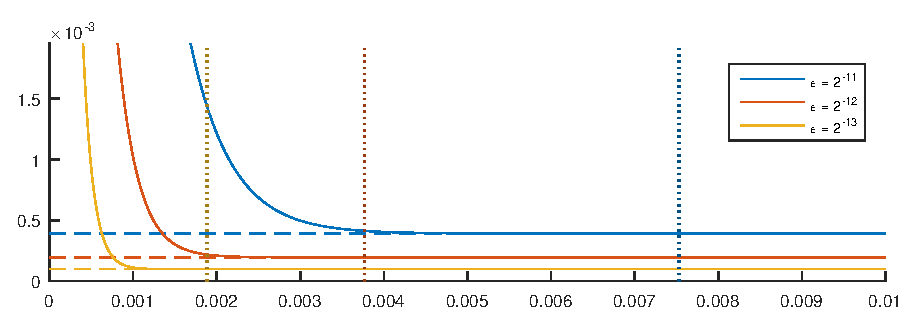
\includegraphics[width=.85\textwidth]{img/chap1/solution_transition_v2.eps}
\caption{Solution $z$ en fonction du temps et la solution sur la variété associée $z_{\infty}:t\mapsto \epsilon h\eeps \circ \varphi_t(x_0\eeps)$, pour $\epsilon = 2^{-11},2^{-12},2^{-13}$. La fin du régime transitoire est indiquée en pointillés comme l'instant $t_0$ à partir duquel $\forall t\geq t_0,\ |z(t)-z_{\infty}(t)| \leq 10^{-8}$.}
\end{figure}

On observe bien dans cet exemple une convergence exponentielle de $z$ vers le régime permanent qu'est la variété centrale $z_{\infty} = \epsilon h\eeps(x)$, avec un régime transitoire de durée d'ordre $\epsilon$. 
En effet on voit que diviser $\epsilon$ par 2 divise également la durée du régime transitoire par 2. 
Il y a bien deux dynamiques en jeu: celle du régime transitoire, en $e^{-t/\epsilon}$ et celle du régime permanent, qui dépend de $\epsilon$ de façon \textit{non raide}. \\


\subsection{Méthodes numériques usuelles} \label{subsec:meth_num_usuelles}

On considère ici principalement les méthodes numériques à pas de temps uniforme. 
On suppose dans nos exemples que le système \eqref{pb:EDO_var_cent} admet une solution bornée sur $[0,T]$, et on définit le pas de temps $\dt = T/N$ avec $N$ le nombre de sous-divisions de l'intervalle. On note $t_n = n\dt,\ n=0,\ldots,N$. 
Pour un schéma donné, on s'intéressera aux erreurs locales $\lex_{n+1}, \lez_{n+1}$ définies par 
$$ \lex = |x_1 - x(\dt)|, \quad \lez = |z_1 - z(\dt)| $$
où $|\cdot|$ est la norme euclidienne de $\R^n$ ou de $\R^m$ et $x_1,z_1$ sont obtenus par le schéma à partir de $x_0,z_0$. 

Les méthodes numériques usuelles à pas fixe permettent d'obtenir des erreurs en $\Delta t^p/\epsilon^q$, $p,q > 0$. 
Lors de la première partie de mon stage, j'ai implémenté et expérimenté avec quelques uns de ces schémas. 
J'ai aussi évalué les performances d'un schéma implicite-explicite \textit{ad hoc}, d'un splitting de Strang et d'un schéma à pas de temps adaptatif. 

On présente certains de ces schémas de façon plus poussée en annexe \ref{chap:erreus_schemas}, avec des études théoriques et numériques d'erreurs. 
En particulier, des graphes d'erreurs sont disponibles. 

\subsubsection{Schémas explicites à pas fixe}

L'erreur locale $\ell e^{(x)}, \ell e^{(z)}$ d'un schéma d'Euler explicite avec $\epsilon < 1$ fixé est 
$$ \lex = \O(\dt^2/\epsilon), \qquad \lez = \O(\dt^2/\epsilon^2). $$ 
Il est intéressant de noter que cela ne génère pas nécessairement une erreur finale en $\epsilon^{-2}$ sur $z$, puisque $z$ cesse rapidement d'être raide. 

\subsubsection{Implicite-explicite \textit{ad hoc}}

Une idée qui peut sembler naturelle est d'impliciter la partie raide pour garder explicite la partie non-linéaire (dans $f,g$). 
Nos calculs et simulations (en annexe \ref{sec:ann_schemas_sep_vitesses}) donnent les erreurs locales 
$$ \lex = \left\{ \begin{array}{ll} 
\O(\dt) &\quad \text{si } \epsilon\ll\dt \\ 
\O(\dt^2/\epsilon) &\quad \text{si } \dt\ll\epsilon 
\end{array} \right. ,
\qquad \lez = \left\{ \begin{array}{ll} 
\O(\epsilon/\dt) &\quad \text{si } \epsilon\ll\dt \\
\O(\dt^2/\epsilon^2) &\quad \text{si } \dt\ll\epsilon
\end{array} \right. $$
On voit qu'il faut toujours imposer $\dt\ll\epsilon$ pour avoir une erreur raisonnable. 
L'avantage est que le schéma est bien plus stable que le schéma complètement explicite, et il est aussi plus rapide qu'un schéma d'Euler implicite usuel. 

\subsubsection{Splitting de Strang}

La partie raide du système est essentiellement contenue dans le terme $-\inveps z$, et donc on propose de séparer le système en deux parties pour le splitting 
$$ \left\{\begin{array}{rl}
\dot x = & 0 \\ \dot z =& -\inveps z
\end{array}\right. \qquad\qquad 
\left\{\begin{array}{rl}
\dot x = & f(x,z) \\ \dot z =& g(x,z)
\end{array}\right. $$
On voit qu'on peut résoudre la première partie exactement à moindre coût, et la deuxième avec un schéma Radau IIA avec une tolérance faible. 
On peut alors supposer que l'erreur provient uniquement du splitting, et donc on calcule une erreur locale théorique d'ordre $\O(\dt^3/\epsilon^2)$ sur $(x,z)$ dans le cas $f,g$ linéaires. 
Cette vitesse de convergence est bien vérifiée pour $x$ sur nos exemples, mais l'ordre est dégénéré pour $z$ (sûrement à cause des non-linéarités). 
Ainsi on obtient 
$$ \lex = \O(\dt^3/\epsilon^2) \qquad \text{et} \qquad 
\lez = \O(\dt^2/\epsilon) $$
Les erreurs globales $e^{(x)},e^{(z)}$ respectent 
$$ e^{(x)} = \O(\dt^2/\epsilon) \qquad \text{et} \qquad e^{(z)} = \O(\dt^2/\epsilon^2) $$
ce qui est bien une convergence d'ordre 2. 


\subsubsection{Pas de temps adaptatif}

Une dernière méthode usuelle que nous avons considérée est une méthode de Runge-Kutta imbriqués d'ordre 3, à partir de RK4 avec la règle des 3/8. Son tableau de Butcher est donné par 
\begin{center}
\begin{tabular}{c|ccccc}
 0  &  0   &  0  &  0  &  0  &  0  \\
1/3 & 1/3  &  0  &  0  &  0  &  0  \\
2/3 & -1/3 &  1  &  0  &  0  &  0  \\
 1  &  1   & -1  &  1  &  0  &  0  \\
 1  & 1/8  & 3/8 & 3/8 & 1/8 &  0  \\ \hline
    & 1/8  & 3/8 & 3/8 & 1/8 &  0  \\ 
    & 1/12 & 1/2 & 1/4 &  0  & 1/6
\end{tabular}
\end{center}
qui nous donne deux estimations $\hat{x}_{n+1},\hat{z}_{n+1}$ et $\tilde{x}_{n+1},\tilde{z}_{n+1}$ (notons que la colonne des coefficients en temps à gauche n'est pas utile dans notre cas). On calcule la différence entre ces deux estimations pour obtenir un pas de temps adapté  
$$ \dt_{\text{opt}} = 0.9 \dt \left(\dfrac{Tol}{|\hat{u}_{n+1}-\tilde{u}_{n+1}|}\right)^{1/4} $$
où $u = \begin{pmatrix} x \\ z \end{pmatrix}$. \\

Ce choix de pas de temps est classique et est présenté à maintes reprises dans \cite{hairer1991}. 
Le cas échéant, il est expliqué en annexe \ref{subsec:ann_rke}. 
Après implémentation, on observe un coût en $\O(1/\epsilon)$ indépendant du facteur de tolérance pour $\epsilon$ petit (fig. \ref{fig:cout_rke} en sec. \ref{subsec:ann_rke}), ce qui rend finalement ce schéma aussi (mal) adapté que les autres. 


\subsubsection{Schéma Radau IIA}
On utilise ce schéma implicite à pas de temps adaptatif pour calculer nos solutions de référence. 
Pour l'implémentation, on utilise un code \bsc{Matlab} \cite{codeRADAU} qui est une traduction du code \bsc{Fortran} de E. Hairer et G. Wanner appliquant la méthode Radau IIA \cite[\textit{sec}.~IV.5]{hairer1991}.

On se sert de ce code pour calculer nos solutions de références et on n'évalue pas sa convergence, mais on peut mesurer son coût en fonction de $\epsilon$. 
\begin{figure}[!h]
\centering
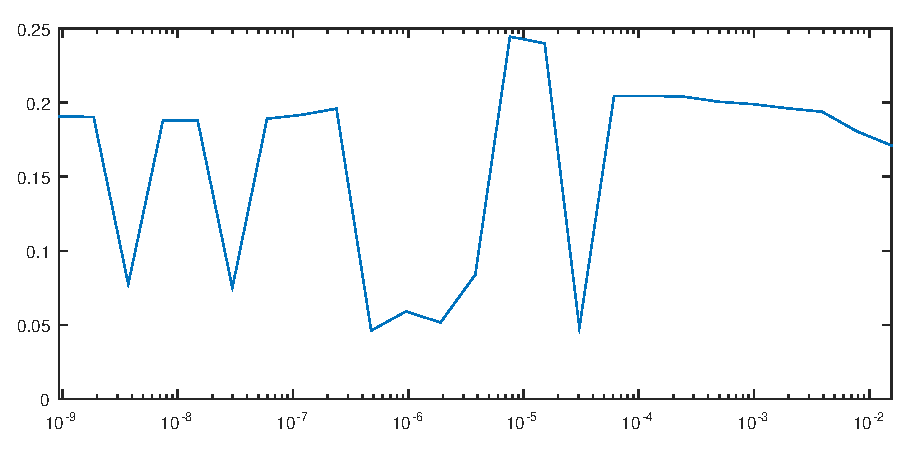
\includegraphics[width=.8\textwidth]{img/chap1/cost_radau.eps}
\caption{Temps du calcul d'une solution $u\eeps$ de référence avec le schéma Radau IIA pour différentes valeurs de $\epsilon$.}
\end{figure}
Il est évident que la valeur de $\epsilon$ a une influence sur le temps de calcul, mais il est impossible de déceler une relation nette. 

On pourrait se dire que ce schéma est suffisant, mais nous allons poursuivre notre étude dans une autre direction pour 
\begin{enumerate}
\item essayer de trouver des méthodes au coût indépendant de $\epsilon$ et
\item trouver des méthodes \textit{uniformément précises} qui pourront nous aider à attaquer d'autres problèmes raides plus complexes par la suite. 
\end{enumerate}


\subsection{Méthodes asymptotiques}

Des méthodes plus modernes et plus formelles cherchent à déterminer l'expression quasi-exacte de la variété $\epsilon h\eeps$ ainsi que la condition initiale modifiée $x_0\eeps$. 

Il est intéressant de noter que $h\eeps$ respecte la relation 
\begin{equation} \label{eq:formule_variete}
\forall x\in\R^n, \qquad \epsilon(h\eeps)'(x)\cdot f(x,\epsilon h\eeps(x)) = - h\eeps(x) + g(x,\epsilon h\eeps(x)) 
\end{equation}
et ainsi, à l'aide de développements limités successifs sur la seconde variable de $f$ et de $g$, on obtient une formulation en puissances de $\epsilon$ pour $h\eeps$. 
En particulier, on a 
$$ h\eeps(x) = g(x,0) + \epsilon \big(\dpz g(x,0)\cdot g(x,0) - \dpx g(x,0)\cdot f(x,0) \big) + \O(\epsilon^2). $$

Il est bien plus difficile de déterminer $x_0\eeps$, puisque cela demande de connaitre l'état du système après la période transitoire pour ensuite <<~remonter~>> le flot de l'équation différentielle réduite \eqref{eq:EDO_reduite}. 
Une méthode a été trouvée récemment dans \cite{castella2016formal} et permet d'obtenir un développement de cette condition modifiée jusqu'à un certain ordre $\epsilon^k$. 
Cette approche est très utile lorsqu'on ne cherche pas à capturer la période transitoire du système et que $\epsilon$ est petit. Elle permet de réduire la complexité du problème \textit{a priori} par principe de réduction (i.e. en se limitant à la variété, où $z$ est déterminé par $x$), et fournit un système dont la seule raideur provient de $f$. Cependant, elle est difficile à implémenter du fait de sa nature algébrique complexe, et n'est pas adaptée si l'on veut capturer la phase transitoire dans une simulation. 

On obtient néanmoins une erreur en $\O(\dt^p + \epsilon^q)$ sur $(x,z)$ après la phase transitoire. \\

Dans \cite{castella2016formal}, la méthode permet également de trouver un nouveau modèle asymptotiquement stable où $x$ est indépendante, peu raide et où on peut calculer $z$ avec le nouveau modèle. 
L'équation sur $z$ peut être raide, en revanche, et les calculs restent assez formels et complexes.
On utilise les résultats de cet article en annexe \ref{subsec:ann_asymp} pour vérifier que l'erreur est la bonne et pour illustrer cette approche. 



\section{Introduction au développement double-échelle}


De la même manière que pour le cas périodique dans \cite{chartier2015UA}, on considère $u = (x,z)$ comme évaluation particulière d'une fonction $U = (X,Z)$ à deux variables $t,\tau$, 
$$ u(t) = U(t,t/\epsilon) $$
pour laquelle on doit trouver un bon ensemble de définition. 
Cette décomposition est aussi à la base de la méthode d'homogénéisation. 
Dans le cas périodique de période $P$, il était naturel de faire évoluer la seconde variable $\tau$ dans $\R/P\mathbb{Z}$, puisqu'elle représentait la partie périodique du problème. 
On verra quel ensemble choisir ici. 

Quel que soit cet ensemble, on trouve que $X,Z$ sont solutions d'un problème de transport 
\begin{equation} \label{eq:trsp_XZ}
\begin{array}{c} \displaystyle
\dpt X + \inveps \dptau X = f(X,Z) 
\\ \displaystyle
\dpt Z + \inveps \dptau Z = -\inveps Z + g(X,Z)
\end{array}
\end{equation}
où la seule donnée qu'on connaît est $X(0,0) = x_0$ et $Z(0,0) = z_0$. \\

On va d'abord discuter des conditions supplémentaires dont on a besoin pour que le problème soit bien posé avec $\tau$ dans un intervalle ou ensemble qu'on choisira, puis on exhibera des conditions pour que le problème soit bien posé et que sa solution soit d'une certaine régularité qu'on précisera. 


\subsection{Nouvelles problématiques}

Comme nous l'avons déjà remarqué, la première difficulté qui se pose est de choisir l'ensemble de définition pour $\tau$. 
Ce choix est en réalité assez simple. 
Dans le cas périodique, l'ensemble de définition de $\tau$ était indépendant de $\epsilon$. 
On souhaite garder cette propriété dans le cas non-périodique, et on observe que si $x,z$ sont définies sur $[0,T]$, $\tau$ parcourt $[0,T/\epsilon]$. 
Ainsi on choisit $\R_+$ comme ensemble pour $\tau$, i.e. on aimerait que $U$ soit définie sur $[0,T]\times\R_+$, i.e. 
$$ U : [0,T]\times\R_+ \rightarrow E := \R^n\times\R^m . $$

On peut maintenant analyser le problème \eqref{eq:trsp_XZ} dans $[0,T]\times\R_+$. 
Il s'agit d'un problème de transport à vitesse constante $1/\epsilon$, donc l'analyse se fera surtout par méthode des caractéristiques. 
Considérons dans un premier temps un problème indépendant de $\epsilon$, 
$$ \dpt u + \dptau u = F(t,\tau,u) $$
avec $F:[0,T]\times\R_+\times E \rightarrow E$. 
On voit qu'on peut obtenir un problème similaire à partir de \eqref{eq:trsp_XZ} avec le changement de variable $\tau \leftarrow \epsilon\tau$, et en fixant $\epsilon$ pour obtenir $F$ indépendante de $\epsilon$. 
Ce problème est donc, à $\epsilon$ fixé, plus général que celui sur $X,Z$. \\


L'aspect de $[0,T]\times\R_+$ fait qu'on doit s'intéresser tout particulièrement à la droite $(t,t),t\in[0,T]$. 
Les droites caractéristiques sont de la forme $(t,\tau+t),\tau\in\R_+,t\in[0,T]$ sous cette diagonale et $(t+t_0, t),t_0\in[0,T],t\in[0,T-t_0]$ au dessus. 
On voit ainsi que certaines caractéristiques ont leur origine sur la demi-droite $(0,\tau),\tau\geq 0$ et d'autre sur le segment $(t_0,0),t_0\in[0,T]$, 
donc pour pouvoir résoudre le problème il faut nécessairement une condition initiale \textit{et} une condition au bord. 

C'est une différence majeure avec le problème périodique, qui ne nécessitait pas de condition au bord. 
Sans condition au bord, la régularité de la condition initiale est transmise naturellement à la solution. Nous allons voir très rapidement que ce n'est pas le cas ici. 
Considérons le problème avec une régularité presque minimale \\
\textit{Trouver $(\overline{T},u)\in]0,T]\times C^0([0,\overline{T}]\times\R_+)$ tel que pour tout $(t,\tau)\in[0,\overline{T}]\times\R_+$ on ait }
\begin{equation} \label{pb:trsp_u_no_eps}
\dpt u + \dptau u = F(t,\tau,u) 
\end{equation}
avec les conditions initiales $u(0,\tau) = u_I(\tau), \tau\in\R_+$ et les conditions au bord $u(t,0) = u_B(t), t\in]0,\overline{T}]$. 
La restriction à $\overline{T} \leq T$ permet d'assurer qu'on ne cherche pas nécessairement une solution sur $[0,T]\times\R_+$ entier, où l'existence ne serait pas toujours garantie à cause des non-linéarités de $F$. 

Admettons qu'on choisisse $u_I$ et $u_B$ quelconques dans $C^0(\R_+)$ et $C^0([0,T])$ respectivement. 
Il est évident que si $u_I(\tau = 0) \neq u_B(t=0)$, la solution (si elle existe) ne peut pas être continue, puisqu'alors $\lim_{\delta\rightarrow 0^+} u(\delta,0) \neq u(0,0)$. 
Réciproquement, 
\begin{lemma} \label{thm:pb_gen_bien_pose}
Si $u_B\in C^0_b([0,T])$, $u_I \in C^0_b(\R_+)$ avec $u_B(t=0) = u_I(\tau = 0) =: u_0$, si $F$ est localement lipschitzienne par rapport à $u$, continue de $[0,T]\times\R_+\times E$ dans $E$, bornée par rapport à $\tau$, alors le problème \eqref{pb:trsp_u_no_eps} est bien posé au sens suivant: 
 
Pour tout facteur $\kappa > 1$, il existe un temps $\Tk\in]0,T]$ tel que le problème (\ref{pb:trsp_u_no_eps}) a une unique solution $u$ dans $C^0([0,\Tk]\times\R^+)$, qui respecte l'inégalité 
\begin{equation}
\forall t\in [0,T_{\kappa}], \qquad \|u(t,\cdot) \|_{\Linftau} \leq \kappa\, \max\left\{ \|u_I\|_{\Linftau}, \|u_B\|_{\Linft} \right\}. 
\end{equation}

Si en outre $F$ respecte $\forall (t,\tau,u)\in [0,T]\times\R_+\times E, |F(t,\tau,u)| \leq C_F |u| + D_F$ pour des constantes $C_F,D_F \geq 0$, alors il existe une unique solution $u$ dans $C^0([0,T]\times\R_+)$ qui vérifie 
\begin{equation}
\forall t\in[0,T], \|u(t,\cdot)\|_{\Linftau} \leq \left( \max\left\{ \|u_I\|_{\Linftau}, \|u_B\|_{\Linft} \right\} + t D_F \right) e^{t C_F}. 
\label{eq:ineg_lin_u}
\end{equation}

\end{lemma}

\begin{proof}
La preuve utilise les droites caractéristiques du problème et ne pose pas de difficultés particulières. 
Néanmoins, sa bonne compréhension nécessite de séparer les fonctions caractéristiques qui ont comme origine une condition initiale de celle qui prennent une condition au bord. 
Cette distinction rend la preuve un peu longue et elle se trouve donc en annexe \ref{chap:ann_preuve}, p. \pageref{chap:ann_preuve}. 
\end{proof}

Exhibons maintenant des conditions supplémentaires sur $u_B$ et $u_I$ pour que la solution $u$ du problème soit de classe au moins $C^2$. 

\subsection{Caractère bien posé dans $C^2$} \label{subsec:carac_C2_gen}

Pour simplifier l'étude, on suppose maintenant $F$ indépendante de $t,\tau$, i.e. $F:E\rightarrow E$. 
Avec $\kappa$ fixé, quitte à ce que ce soit au sens des distributions dans $L^{\infty}([0,\Tk]\times\R_+)$, on peut dériver le problème de transport \eqref{pb:trsp_u_no_eps} selon $t$ pour obtenir que $\dpt u\eeps =: v\eeps$ vérifie 
\begin{equation} 
\begin{array}{c}
\displaystyle
\dpt v + \dptau v = \dpu F(u)\cdot v \vphantom{\int_0^1}
\\ \displaystyle
v(0,\tau) = F(u_I(\tau)) - u_I'(\tau) \quad \text{et} \quad v(t,0) = u_B'(t)
\end{array}
\label{pb:trsp_v_no_eps}
\end{equation}
D'après l'étude précédente, il apparaît immédiatement que pour que $v$ soit continue, il faut non seulement avoir $u_I\in C^1(\R_+)$, $u_B\in C^1([0,\Tk])$  
et $\dpu F$ continue de $E$ dans $L(E,E)$, mais aussi 
\begin{equation}
u_B'(t=0) + u_I'(\tau = 0) = F(u_0)
\label{eq:compat_ord1}
\end{equation}
où $u_0 := u_I(\tau = 0) = u_B(t = 0)$. 
Admettons que nos conditions initiale et au bord sont bien choisies de sorte que $v$ ainsi définie soit continue (i.e. de sorte que la relation \eqref{eq:compat_ord1} soit vérifiée). 
Alors on peut dériver à nouveau pour obtenir une équation sur $\dpt v =: w$ 
\begin{equation} \label{pb:trsp_w_no_eps}
\begin{array}{lc}
&\displaystyle
\dpt w + \dptau w = %\dpt^2 F(t,\tau,u) + \dpt\dpu F(t,\tau,u) +
\dpu^2 F(u)\cdot (v,v) + \dpu F(u)\cdot w \vphantom{\int_0^1}
\\ & \displaystyle
w(0,\tau) = %\dpt F_0(\tau,u_I) + 
\dpu F(u_I)\cdot (v(0,\tau) - u_I') %- \dptau F_0(\tau,u_I) 
+ u_I'' \vphantom{\int_0^1} 
\quad %\\
\text{et} \quad w(t,0) = u_B''(t)
\end{array}
\end{equation}
où %$F_0(\cdot,\cdot) = F(0,\cdot,\cdot)$ et 
$u_I,u_I'$ et $u_I''$ sont évaluées en $\tau$ dans la condition initiale. On voit que la condition de continuité peut alors s'écrire 
\begin{equation} \label{eq:compat_ord2} 
%\dpt F(0,0,u_0) + 
\dpu F(u_0)\cdot u_B'(0) - u_B''(0) = %\dptau F(0,0,u_0) + 
\dpu F(u_0)\cdot u_I'(0) - u_I''(0). 
\end{equation}
On peut alors exhiber des conditions suffisantes pour que la solution soit de classe $C^2$ dans le problème \eqref{pb:trsp_u_no_eps}, avec $F$ indépendante de $t,\tau$. \\


\begin{theorem} \label{thm:regularite_u_no_eps}
Si $u_B\in C^2_b([0,T])$, $u_I\in C^2_b(\R_+)$, 
si $F$ (resp. $\dpu F$ et $\dpu^2 F$) est continue de $E$ dans $E$ (resp. $L(E,E)$ et $L(E^2,E)$), et enfin si 
$$u_B(0) = u_I(0) =: u_0, \qquad u_B'(0) + u_I'(0) = F(u_0),$$
$$ \text{et}\quad %\dpt F(0,0,u_0) + 
\dpu F(u_0)\cdot u_B'(0) - u_B''(0) = %\dptau F(0,0,u_0) + 
\dpu F(u_0)\cdot u_I'(0) - u_I''(0) $$
alors le problème \eqref{pb:trsp_u_no_eps} est bien posé et régulier au sens suivant :

Pour tout facteur $\kappa > 1$, il existe un temps $\Tk\in]0,T]$ tel que le problème (\ref{pb:trsp_u_no_eps}) a une unique solution $u$ dans $C^2([0,\Tk]\times\R^+)$, qui respecte l'inégalité 
\begin{equation}
\forall t\in [0,T_{\kappa}], \qquad \|u(t,\cdot) \|_{\Linftau} \leq \kappa\, \max\left\{ \|u_B\|_{\Linft}, \|u_I\|_{\Linftau} \right\}. 
\label{eq:ineg_u_no_eps}
\end{equation}
et avec $C_0' = \sup\left\{\vertiii{\dpu F(u(t,\tau))},\, (t,\tau)\in [0,\Tk]\times\R_+ \right\}$ on a 
\begin{equation}
\forall t\in[0,\Tk], \qquad \|\dpt u(t,\cdot)\|_{\Linftau} \leq \max \left\{\|u_B'\|_{\Linft}, \|v_I\|_{\Linftau} \right\} e^{t C_0'},
\end{equation}
où $v_I = F(u_I) - u_I'$. De la même manière, avec $C_1'' = \| \dpu^2 F(u)\cdot(v,v )\|_{L_{t,\tau}^{\infty}}$, on a 
\begin{equation}
\forall t\in[0,\Tk], \qquad \|\dpt^2 u(t,\cdot)\|_{\Linftau} \leq \left( \max \left\{\|u_B''\|_{\Linft}, \|w_I\|_{\Linftau} \right\} + t C_1'' \right) e^{t C_0'}
\end{equation} 
où $w_I = \dpu F(u_I)\cdot(v_I - u_I') + u_I''$. 
\end{theorem}

\begin{proof}
Soit $\kappa > 1$. Le lemme \ref{thm:pb_gen_bien_pose} assure l'existence de $(\Tk,u)\in ]0,T]\times C^0_b([0,\Tk]\times\R_+)$ vérifiant l'inégalité souhaitée. 
On peut ensuite appliquer le cas affine du lemme \ref{thm:pb_gen_bien_pose} successivement aux problèmes \eqref{pb:trsp_v_no_eps} puis \eqref{pb:trsp_w_no_eps} en considérant $u$ puis $v$ comme des paramètres, et on obtient $\dpt u \in C^0_b([0,\Tk]\times\R_+)$ puis $\dpt^2 u\in C^0_b([0,\Tk]\times\R_+)$), avec les bornes souhaitées. 

On remarque enfin 
$$\dptau u = F(u) - \dpt u, \quad\dptau \dpt u = \dpu F(u)\cdot \dpt u - \dpt^2 u \quad\text{et}\quad \dptau^2 = \dpu F(u)\cdot \dptau u - \dpt \dptau u$$
donc la régularité de $u,\dpt u$ et $\dpt^2 u$ se propage aux dérivées première et seconde de $u$ pour assurer $u\in C^2([0,\Tk]\times\R_+)$. 

\end{proof}

On voit ainsi que les conditions initiale et au bord sont intimement liées. 
Puisqu'on est libre de choisir les deux, on se dit que le plus simple est de fixer l'une des deux pour ensuite choisir l'autre de manière adaptée. 
On choisit de se concentrer d'abord sur la condition initiale, pour des raisons qui vont apparaître rapidement. 

\begin{remark}
Pour avoir une solution d'ordre $C^3$, on doit respecter 
$$
u_B''' + u_I''' = \dpu^2 F(u_0)\cdot(u_B',u_B') + \dpu^2 F(u_0)\cdot(u_I',u_I') - \dpu^2 F(u_0)\cdot(u_B',u_I') + \dpu F(u_0)\cdot(u_B''+u_I'') .
$$
\end{remark}

\subsection{Condition initiale ou condition au bord?}

Le but est de trouver de bonnes données (conditions initiale et au bord) de sorte à avoir $X,\dpt X, \dpt^2 X$ et $Z,\dpt Z, \dpt^2 Z$ uniformément bornés sur $[0,\Tk]\times\R_+$ afin de pouvoir trouver un schéma numérique uniformément précis (UP) d'ordre 1, i.e. d'erreur globale $\O(\dt)$ à constante indépendante de $\epsilon$. 
L'inspiration provient naturellement des méthodes d'Euler pour lesquelles l'erreur locale est d'ordre $\dt^2 (\|\dpt^2 X\| + \|\dpt^2 Z\|)$. 

Mettons d'abord le problème \eqref{eq:trsp_XZ} sous la forme 
\begin{equation} \label{eq:trsp_U_L}
\dpt U + \inveps LU = F(U) 
\end{equation} 
avec $U = \begin{pmatrix} X \\ Z \end{pmatrix}$ et $F(U) = \begin{pmatrix} f(X,Z) \\ g(X,Z) \end{pmatrix}$, des conditions initiale $U_I$ et au bord $U_B$, et $L$ un opérateur bien choisi. En l'occurrence, 
$$ LU := \begin{pmatrix} L_x X \\ L_z Z \end{pmatrix} := \begin{pmatrix} \dptau X \\ e^{-\tau} \dptau [e^{\tau} Z] \end{pmatrix}. $$
On admet pour le moment qu'on peut borner $\dpt U$ en fonction de $\inveps LU_I$ puisque $\dpt U(0,\tau) = F(U_I) - \inveps LU_I$ et que le lemme \ref{thm:regularite_u_no_eps} va dans ce sens. 
On voit alors qu'un mauvais choix de la condition initiale peut faire apparaître un facteur $1/\epsilon$ dans $\dpt U$. 

On voit en revanche que pour la valeur au bord de $\dpt U$, seule la dérivée $U_B'$ compte: il n'y a pas de facteur $1/\epsilon$ qui apparaît. Même pour les dérivées en $\tau$, on a $\dptau U(t,0) = -U_B + \epsilon(F(U_B) - U_B')$, donc $U_B$ semble ne pouvoir faire apparaître un facteur $1/\epsilon$ que si sa dérivée en fait apparaître un. 

En outre, si $U_I$ est telle que $\dpt U(0,\cdot) =: V_I(\cdot)$ et $\dpt^2 U(0,\cdot) =: W_I(\cdot)$ sont définies (il suffit d'avoir $U_I \in C^2$) et uniformément bornées, i.e. $$\exists C>0,\forall \epsilon\in]0,\epsilon^*], \|V_I\|_{\Linftau},\|W_I\|_{\Linftau} \leq C$$
alors on peut définir 
\begin{equation} \label{eq:CB_UVW}
U_B(t) = U_I(0) + t V_I(0) + \frac 1 2 t^2 W_I(0)
\end{equation}
pour obtenir une solution de classe $C^2$ qui, on l'espère (et on le montrera ensuite), est uniformément bornée sur $[0,T]\times\R_+$ avec ses dérivées $\dpt U, \dpt^2 U$ qui le sont aussi. 
\chapter{Mise en place d'un schéma numérique uniformément convergent}

Maintenant qu'on sait comment obtenir un problème régulier, on cherche des conditions initiales qui permettent d'obtenir une condition au bord uniformément bornée avec la formule \eqref{eq:CB_UVW}. 
On montre ensuite que le problème est alors bien posé et donne $U, \dpt U$ et $\dpt^2 U$ uniformément bornées, et on traduit les conditions initiales et au bord explicitement pour $X,Z$. 
Enfin, on met en place un schéma numérique uniformément convergent dont on prouve les convergences locales et globales. 

Par la suite on ne considère plus la variété centrale $\epsilon h\eeps$, si bien que les notations $h,h\eeps$ pourront représenter n'importe quel type de fonctions. 


\section{Choix de la condition initiale}

Cette section décrit une analyse du problème à l'aide d'outils utiles au cas périodique. 
À cet effet, les méthodes présentées partent d'hypothèses de régularité qui ne sont pas explicitées. 

D'abord on présente une approche peu formelle par développement en puissances de $\epsilon$ qui a fait le sujet d'une bonne partie du stage. 
Face aux limites de cette approche, on exhibe une meilleure méthode pour trouver les bonnes conditions initiales pour avoir des dérivées $\dpt^{\alpha}$ uniformément bornée jusqu'à un ordre $\alpha\in\N$ arbitraire. 
 

\subsection{Approche initiale}

Dans un premier temps, on a essayé de faire le lien entre un développement multi-échelles en puissances de $\epsilon$ et la régularité sous la diagonale. On écrit ce développement 
$$ X\eeps(t,\tau) = \sum_{n\in\N} \epsilon^n X_n(t,\tau) 
\qquad \text{et} \qquad
Z\eeps(t,\tau) = \sum_{n\in\N} \epsilon^n Z_n(t,\tau) $$
en supposant les $X_n$, $Z_n$ et leurs dérivées uniformément bornées en $\epsilon$. \\

Analysons le comportement de la solution approchée $X = X_0, Z = Z_0$. On a par développement selon les puissance de $\epsilon$
\begin{equation*}
\begin{array}{lclr}
\dptau X_0 = 0, &\qquad& \dptau Z_0 + Z_0 = 0 &\qquad \qquad (\epsilon^{-1}) \\
\dpt X_0 = f(X_0,Z_0), &\qquad& \dpt Z_0 = g(X_0,Z_0) &\qquad \qquad (\epsilon^0)
\end{array}
\end{equation*}

La condition initiale associée à ce problème <<~tronqué~>> est alors évidente: on a 
\begin{equation}
X(0,\tau) = x_0, \quad Z(0,\tau) = e^{-\tau}z_0.
\end{equation}
On a alors effectivement $\dpt X(0,\tau) = f(x_0,e^{-\tau}z_0)$ et $\dpt Z(0,\tau) = g(x_0,e^{-\tau}z_0)$, ce qui est uniformément borné sur $\R_+$, mais en dérivant à nouveau on obtient $\dpt^2 X(0,\tau) = \O(1/\epsilon)$ et $\dpt^2 Z(0,\tau) = \O(1/\epsilon)$. 

On tronque maintenant à l'ordre $1$: $X = X_0 + \epsilon X_1, Z = Z_0 + \epsilon Z_1$. Comme précédemment, on a 
\begin{equation*}
\begin{array}{lclr}
\dptau X_0 = 0, &\qquad& \dptau Z_0 + Z_0 = 0 &\qquad \qquad (\epsilon^{-1}) \\
\dptau X_1 = f(X_0,Z_0) - \dpt X_0, &\qquad& \dptau Z_1 + Z_1 = g(X_0,Z_0) - \dpt Z_0 &\qquad \qquad (\epsilon^0) \\
\dpt X_1 = \Delta_{\epsilon}f(X_0,Z_0)\cdot (X_1,Z_1), &\qquad& \dpt Z_1 = \Delta_{\epsilon}g(X_0,Z_0)\cdot(X_1,Z_1) &\qquad \qquad (\epsilon^1)
\end{array}
\end{equation*}
où $\Delta_{\epsilon} f(X_0,Z_0)\cdot(X_1,Z_1) = \dfrac{1}{\epsilon}[f(X_0 + \epsilon X_1, Z_0 + \epsilon Z_1) - f(X_0, Z_0)] = f_x(X_0,Z_0)\cdot X_1 + f_z(X_0,Z_0)\cdot Z_1 + \O(\epsilon)$, une sorte de dérivée discrète. \\

Puisque $X(0,0)$ et $Z(0,0)$ sont fixés comme indépendant de $\epsilon$, on pose $X_1(0,0) = 0$ et $Z_1(0,0) = 0$. 
Alors on a toujours $X_0(t,\tau) = x_0(t), Z_0(t,\tau) = e^{-\tau}z_0(t)$ (avec l'abus de notation où $x_0,z_0$ sont des fonctions du temps qui coïncident avec leur définition précédente en 0), mais aussi 
\begin{equation*}
\begin{array}{l}
\displaystyle
X_1(t,\tau) = \int_0^{\tau} \Big[f\big(x_0(t),e^{-\sigma}z_0(t)\big) - \dot{x_0}(t)\Big] d\sigma + x_1(t) \\
\displaystyle
Z_1(t,\tau) = \int_0^{\tau} e^{-(\tau-\sigma)}\Big[g\big(x_0(t),e^{-\sigma}z_0(t)\big) - e^{-\sigma}\dot{z_0}(t)\Big]d\sigma + e^{-\tau}z_1(t)
\end{array}
\end{equation*}
avec $x_1(0) = 0, z_1(0) = 0$ et $\dot{x_1},\dot{z_1}$ donnés par le système d'ordre $\epsilon^1$ (ces fonctions n'influencent de toute manière pas les conditions initiales). 

On voit qu'on n'a pas encore de relation pour $\dot{x_0}$ ni $\dot{z_0}$. On peut cependant en extraire une pour $\dot{x_0}$. 
En effet, puisqu'on veut avoir $X_1$ bornée, il faut nécessairement $\dot{x_0} = f(x_0,0)$. 
Le choix de $\dot{z_0}$, est arbitraire, et on voit par le calcul que quel que soit notre choix, on obtient une condition initiale et des dérivées $X,\dpt X, \dpt^2 X$ et $Z,\dpt Z, \dpt^2 Z$ uniformément bornées sur $(0,\tau),\tau > 0$. \\

Lorsqu'on veut étendre le développement à l'ordre 2 en $\epsilon$, i.e. $X = X_0 + \epsilon X_1 + \epsilon^2 X_2$ et $Z = Z_0 + \epsilon Z_1 + \epsilon^2 Z_2$, on se rend compte que les calculs deviennent plus compliqués et qu'on a encore beaucoup de choix à faire sur $\ddot{x_0},\ddot{z_0},\dot{x_1},\dot{z_1}$. 
On va donc chercher un cadre formel qu'on pourra utiliser pour trouver des conditions initiales permettant d'avoir des $\dpt^{\alpha} X(0,\tau), \dpt^{\alpha} Z(0,\tau)$ uniformément bornées jusqu'à $\alpha$ arbitraire. 


\subsection{Développement de Chapman-Enskog}

On reprend la formulation \eqref{eq:trsp_U_L}:
$$ \dpt U + \inveps LU = F(U). $$

\'{E}tudions l'opérateur $L$ dans l'ensemble $\E = \big\{h:\R^+ \rightarrow E \,|\, \exists (h_n)_{n\in\N}, \forall\tau\in\R^+, h(\tau) = \sum_n h_n e^{-n\tau}\big\}$, l'ensemble des séries exponentielles. 
Cet ensemble est plus contraignant que les preuves suivantes ne le nécessitent, mais cela rendra les raisonnement plus clairs, et est en accord avec l'analogie des fonctions périodiques qui sont aussi des séries, de la forme $\sum_n h_n e^{in\tau}$. 
Pour assurer que $\E$ est stable par $F$, on suppose $F$ analytique. 

Les noyaux de $L_x$ et $L_z$ sont respectivement $Vect(\tau\mapsto 1_{\R^n})$ et $Vect(\tau\mapsto e^{-\tau}1_{\R^m})$. 
On note $\Pi_x$ et $\Pi_z$ les projections sur ces noyaux. Sur le complémentaire des noyaux respectifs de $L_x$ et $L_z$ (i.e. sur les noyaux respectifs de $\Pi_x$ et $\Pi_z$), on a 
\begin{equation*}
\begin{array}{rl}
(L_x^{-1} a)(\tau) =& \displaystyle
-\int_{\tau}^{\infty} a(\sigma)d\sigma = (I - \Pi_x) \int_0^{\tau} a(\sigma)d\sigma , \\
(L_z^{-1} b)(\tau) =& \displaystyle
b_0 - \int_{\tau}^{\infty}e^{-\tau+\sigma} (b(\sigma) - b_0)d\sigma = (I - \Pi_z) \int_0^{\tau} e^{-\tau+\sigma}b(\sigma)d\sigma .
\end{array}
\end{equation*}
Il est intéressant de remarquer qu'on doit modifier un peu l'intégrande pour pouvoir définir l'inverse de $L_z$. 
En définissant $o_x : \tau \mapsto 1_{\R^n}$ et $o_z : \tau\mapsto e^{-\tau}1_{\R^m}$ les fonctions de base de $\text{Ker } L_x$ et $\text{Ker } L_z$ respectivement, on remarque 
$$ (L_x^{-1} a)(\tau) = (I - \Pi_x) (o_x * a), $$
$$ (L_z^{-1} b)(\tau) = (I - \Pi_z) (o_z * b). $$
où $*$ représente le produit de convolution. 
De manière générale, si $Th = e^{-p\tau}\dptau[e^{p\tau}h]$ avec $h = \sum_{k\neq p} h_k e^{-k\tau} \in \E /\,\text{Ker }T $ on inverse $(T^{-1}h)(\tau) = \sum_{k \neq p} \frac{1}{p-k}h_k e^{-k\tau} = \sum_{k < p} \frac{1}{p-k}h_k e^{-k\tau} - \int_{\tau}^{\infty} e^{-k(\tau-\sigma)}\big( h(\sigma) - \sum_{k < p}h^k e^{-k\sigma} \big)d\sigma$.  \\

Supposons connaître la solution $U\eeps$. %\unsure{Techniquement il faudrait avoir $U\eeps(t,\cdot)\in\E$ pour tout $t$, mais c'est pas le cas... Je viens de m'en rendre compte. On s'en sort comment?} 
Le développement de Chapman-Enskog consiste à la décomposer en deux parties 
$$ U\eeps(t,\tau) = \underline{U}\eeps(t,\tau) + h\eeps(t,\tau) $$
où $\underline{U}\eeps := \Pi U\eeps$ et $\Pi h\eeps = 0$ (on rappelle que $h\eeps$ n'est pas la variété du théorème \ref{thm:var_cent}). 
On peut injecter cette décomposition de $U\eeps$ dans le système de départ, puis projeter sur le noyau de $L$ pour obtenir les équations 

$$\dpt \underline{U}\eeps = \Pi F(\underline{U}\eeps+h\eeps), $$
$$\dpt h\eeps + \inveps Lh\eeps = (I-\Pi)F(\underline{U}\eeps+h\eeps). $$

Comme $\Pi h\eeps = 0$ on déduit de la dernière relation 

$$ h\eeps = \epsilon A F(\underline{U}\eeps+h\eeps) - \epsilon L^{-1}(\dpt h\eeps). $$
avec $A := L^{-1}(I-\Pi)$ (défini sur $\E$ tout entier). En supposant $U\eeps$ suffisamment régulière, on peut décomposer $h$ en puissances de $\epsilon$:
$$ h\eeps(t,\tau) = \epsilon h_1(t,\tau,\underline{U}\eeps) + \epsilon^2 h_2(t,\tau,\underline{U}\eeps) + \ldots $$

Et alors en supposant $h\eeps, \dpt h\eeps = \O_{\epsilon\rightarrow 0}(1)$ on obtient $h\eeps = \O(\epsilon)$. Si on suppose en outre $\dpt^2 h\eeps = \O(1)$ on obtient 
$$ h\eeps = \epsilon h_1 + \O(\epsilon^2) := \epsilon AF(\underline{U}\eeps) + \O(\epsilon^2). $$

\newcommand{\ulU}{\underline{U}}
\newcommand{\ulX}{\underline{X}}
\newcommand{\ulZ}{\underline{Z}}
\newcommand{\ulx}{\underline{x}}
\newcommand{\ulz}{\underline{z}}
\newcommand{\ulf}{\underline{f}}
\newcommand{\ulg}{\underline{g}}

On s'attend à avoir une solution régulière à l'ordre 2 si les conditions initiales respectent ce développement $U_0 = \underline{U}_0 + \epsilon h_1$, c'est-à-dire avec 
\begin{equation}
U_0\eeps(\tau) = \underline{U}_0\eeps(\tau) + \epsilon A F(\underline{U}_0\eeps(\tau)).
\label{eq:CI_chapman}
\end{equation}
où $\ulU_0\eeps = \Pi \ulU_0\eeps = \Pi U_0\eeps$ pourra être déterminé à partir de $U_0\eeps(0,0) = u_0$ (seul degré de liberté qui correspond aux conditions initiales du problème \eqref{pb:EDO_var_cent}). 


\begin{remark}
On pourrait aller un ordre au dessus en supposant $\dpt^3 h\eeps = \O(1)$ et alors on obtiendrait 
$$ \begin{array}{rl}
U_0\eeps(\tau) =& \underline{U}_0\eeps(\tau) + \epsilon A F(\underline{U}_0\eeps) \\
+& \epsilon^2 \Big( A\dpu F(\ulU_0\eeps) A F(\ulU_0\eeps) - A^2 \dpu F(\ulU_0\eeps)\Pi F(\ulU_0\eeps) \Big). 
\end{array} $$
\end{remark}



\section{Bornes uniformes de la solution}

L'étude de la régularité en section \ref{subsec:carac_C2_gen} nous indique qu'on peut définir $U_{\alpha}\eeps(\tau) = (\dpt^{\alpha} U\eeps)(0,\tau),\ \alpha = 0,1,2$ à partir de $F$ et des dérivées de $U_0\eeps$. On choisit alors la condition au bord 
%
\begin{equation}
U_B\eeps(t) = U_0\eeps(0) + t\, U_1\eeps(0) + \dfrac{t^2}{2}U_2\eeps(0). 
\label{eq:CB_ord2}
\end{equation}
%
Si $U_0\eeps(0), U_1\eeps(0), U_2\eeps(0) = \O_{\epsilon\rightarrow0}(1)$, alors $U_B\eeps,\dpt U_B\eeps$ et $\dpt^2 U_B\eeps$ sont uniformément bornées sur $[0,T]$. 
Montrons qu'avec ce choix de conditions initiale et au bord, on obtient une solution $U\eeps$ avec les propriétés souhaitées. 

\subsection{Théorème sur $U = (X,Z)$}

\begin{theorem} \label{thm:regu_U}
Considérons le problème de transport (\ref{eq:trsp_U_L}) avec les conditions initiales (\ref{eq:CI_chapman})
$$ U_0\eeps(\tau) = \underline{U}_0\eeps(\tau) + \epsilon L^{-1} (I-\Pi) F(\underline{U}_0\eeps(\tau)) $$
et les conditions au bord (\ref{eq:CB_ord2}). On suppose $F$ analytique. Alors 
\begin{enumerate}[(i)]
\item Les conditions initiales et au bord sont uniformément bornées en norme infinie, et il existe pour tout $\kappa > 1$ un temps $T_{\kappa}$ tel que pour tout $\epsilon\in]0,\epsilon^*]$ une unique solution $U\eeps$ dans $C^2([0,T_{\kappa}]\times\R_+)$ qui vérifie 
\begin{equation} \label{eq:ineg_Ueps}
\forall t\in[0,T_{\kappa}],\quad \sup_{\epsilon\in]0,\epsilon^*]} \| U\eeps(t,\cdot) \|_{L^{\infty}_{\tau}} \leq \kappa \sup_{\epsilon\in]0,\epsilon^*]} \left(\max\left\{ \|U_0\eeps\|_{\Linftau}, \|U_B\eeps\|_{\Linft} \right\} \right) < +\infty . 
\end{equation}

\item Pour tout $\Tk$ assurant l'inégalité \eqref{eq:ineg_Ueps}, il existe une constante $C_{\kappa}$ telle que la solution $U\eeps$ vérifie 
\begin{equation} \label{ineq:dtUeps}
\forall t\in[0,\Tk], \quad \sup_{\epsilon\in]0,\epsilon^*]} \|\dpt^{\alpha} U\eeps(t,\cdot)\|_{L^{\infty}_{\tau}} \leq C_{\kappa}, \quad \alpha = 0,1,2.
\end{equation}
\end{enumerate}
\end{theorem}

\begin{proof}
\newcommand{\ulF}{\underline{F}}
Le théorème \ref{thm:regularite_u_no_eps} nous permet d'affirmer que le problème est bien posé dans $C^2([0,\Tk]\times\R_+)$ à $\epsilon$ et $\kappa$ fixé. La difficulté va être de montrer que $\Tk$ et les bornes peuvent être indépendantes de $\epsilon$. 

\vspace*{7pt}
\noindent {\itshape{}Étude de la condition au bord.\hspace*{.3cm}}
Montrons d'abord que la condition au bord est uniformément bornée (i.e. $\sup_{\epsilon} \|U_B\|_{\Linft} < \infty$). 
On remarque d'abord $U_0\eeps(0) = \O_{\epsilon\rightarrow 0}(1)$ et on calcule 
$$U_1\eeps = F(U_0\eeps) - \inveps LU_0\eeps = F_0\eeps - (I-\Pi)\ulF_0\eeps $$
avec $F_0\eeps = F(U_0\eeps)$ et $\ulF_0\eeps = F(\ulU_0\eeps)$. Cette condition initiale est uniformément bornée, donc on a $U_1\eeps(0) = \O_{\epsilon\rightarrow 0}(1)$. Remanions un peu les termes pour trouver une expression plus simple à dériver. Par développement limité autour de $\ulU_0\eeps$ dans $F(U_0\eeps)$ on trouve 
$$ \begin{array}{rl}
F_0\eeps - \ulF_0\eeps =& \dpu F(\ulU_0\eeps)(U_0\eeps - \ulU_0\eeps) + \O(\|U_0\eeps - \ulU_0\eeps\|^2) \\
=& \epsilon\dpu F(\ulU_0\eeps) A\ulF_0\eeps + \O(\epsilon^2) 
\end{array} $$ 
$$ \text{d'où} \qquad U_1\eeps = \Pi\ulF_0\eeps + \epsilon\dpu F(\ulU_0\eeps) A\ulF_0\eeps + \epsilon^2 r_1\eeps $$
avec le terme correctif $r_1\eeps\in\E$ qui vient prendre en compte le reste dans le développement autour de $\ulU_0\eeps$. On a ensuite 
$$ U_2\eeps = \dpu F(U_0\eeps)\cdot U_1\eeps - \inveps LU_1\eeps = \dpu F(U_0\eeps) - L\dpu F(\ulU_0\eeps) A F(\ulU_0\eeps) + \O(\epsilon)$$
et donc $U_2\eeps(0) = \O_{\epsilon\rightarrow 0}(1)$. On a ainsi montré que $U_0\eeps,U_1\eeps,U_2\eeps$ et $U_B\eeps,(U_B\eeps)',(U_B\eeps)''$ sont uniformément bornées. 

\vspace*{7pt}
\noindent {\itshape{}Existence de $\Tk$ et de $U$, et borne uniforme.\hspace*{.3cm}}
On écrit le problème sous la forme 
$$ \dpt U\eeps + \partial_{\theta} U\eeps = -\inveps J U\eeps + F(U\eeps), $$
avec $J$ diagonale, de coefficients 0 ou 1 selon que le coefficient agisse sur $X$ ou $Z$. 
Ce problème est presque celui de la partie 1 à l'exception du terme $-(1/\epsilon)JU\eeps$ et de l'indépendance de $F$ par rapport à $t,\tau$ (et d'un changement de variable $\tau \leftarrow \epsilon\tau$). 

Soit $\kappa > 1$. 
Montrons que les résultats du lemme \ref{thm:pb_gen_bien_pose} sont maintenus, avec un temps final $\Tk$ et une borne à la solution tous les deux indépendants de $\epsilon$. 

On s'intéresse d'abord aux caractéristiques sous la diagonale pour nous ramener au cas de la partie précédente. 
Soit $\tau \geq 0$, on pose $\varphi\eeps(t,\tau) = U\eeps(t,\tau+t/\epsilon)$, alors $\varphi\eeps(t,\tau)$ vérifie l'EDO 
$$ \dpt \varphi\eeps(t,\tau) = -\inveps J\varphi\eeps(t,\tau) + F(\varphi\eeps(t,\tau)) \quad\text{et}\quad \varphi\eeps(0,\tau) = U_0\eeps(\tau) $$
Sous forme intégrale, le problème s'écrit 
$$ \varphi\eeps(t,\tau) = e^{-tJ}\varphi\eeps(0,\tau) + \int_0^{\tau} e^{(s-t)J} F(\varphi(s,\tau))ds $$
soit, par inégalité triangulaire et croissance de l'intégrale, en remarquant $\vertiii{e^{-tJ}} \leq 1$, 
\begin{equation} \label{ineq:phi_eps}
|\varphi\eeps(t,\tau)| \leq |\varphi\eeps(0,\tau)| + \int_0^{\tau} |F(\varphi(s,\tau))|ds. 
\end{equation}
On est alors exactement dans le même cas que dans la démonstration du lemme \ref{thm:pb_gen_bien_pose} (voir annexe~\ref{chap:ann_preuve}). 
Il en est de même \textit{au dessus} de la diagonale $(t,t/\epsilon)$. Notons $R := \sup_{\epsilon} \max \left\{\|U_0\eeps\|_{\Linftau},\|U_0\eeps\|_{\Linft}\right\}$. 
On peut alors définir un temps final $\Tk$ indépendant de $\epsilon$ tel que $U\eeps$ est bien définie et est bornée par $\kappa R$ sur $[0,\Tk]\times\R_+$ pour tout $\epsilon$. En particulier, on passe au supremum pour obtenir l'inégalité \eqref{eq:ineg_Ueps} du théorème. 

\vspace*{7pt}
\noindent {\itshape{}Continuité et caractère borné des dérivées.\hspace*{.3cm}}
On rappelle que $\dpt U\eeps$ (resp. $\dpt^2 U\eeps$) vérifie un problème de transport linéaire avec pour conditions initiale $U_1$ (resp. $U_2$) et au bord $U_B'$ (resp. $U_B''$). De même que précédemment, on peut montrer que le cas affine du lemme \ref{thm:pb_gen_bien_pose} reste valide, avec une borne indépendante de $\epsilon$. Détaillons le raisonnement pour $\dpt U\eeps =: V\eeps$ afin de s'en convaincre. On a 
$$ \begin{array}{c} \displaystyle
\dpt V\eeps + \inveps\dpt V\eeps = -\inveps J V\eeps + \dpu F(U\eeps)\cdot V\eeps, 
\\ \displaystyle \vphantom{\inveps}
V\eeps(0,\tau) = U_1(\tau) \quad\text{et}\quad V(t,0) = (U_B\eeps)'(t).
\end{array} $$
En notant $G\eeps:t,\tau,v \mapsto \dpu F(U\eeps(t,\tau))\cdot v$, cela s'écrit sous forme intégrale pour une caractéristique $\psi\eeps(t,\tau) = V\eeps(t,\tau+t/\epsilon)$ sous la diagonale, $\psi\eeps(t,\tau) = e^{-\frac{t}{\epsilon}J}\psi\eeps(0,\tau) + \int_0^t e^{\frac{(s-t)}{\epsilon}J} G\eeps(s,\tau+s/\epsilon,\psi\eeps(s,\tau))ds$. 
Comme précédemment, on peut majorer $\psi\eeps(t,\tau)| \leq |\psi\eeps(0,\tau)| + \int_0^t |G\eeps(s,\tau+s/\epsilon,\psi\eeps(s,\tau))|ds$. 

Comme $U\eeps$ est bornée sur $[0,\Tk]\times\R_+$, $\dpu F(U\eeps)$ l'est aussi en norme d'opérateur. 
On pose $A_{\kappa},B_{\kappa} > 0$ tels que $\forall (\epsilon,t,\tau,v)\in ]0,\epsilon^*]\times [0,\Tk]\times\R_+\times E, |G\eeps(t,\tau,v)| \leq A_{\kappa} |v| + B_{\kappa}$ 
(en l'occurrence on pourrait choisir $B_{\kappa} = 0$ mais ce n'est pas le cas pour $\dpt^2 U\eeps$ donc conservons le). L'inégalité de Grönwall assure alors 
$$\forall t\in[0,\Tk], \quad \|V\eeps(t,\cdot)\|_{\Linftau} \leq \left(\max \left\{\|(U_B\eeps)'\|_{\Linft},\|U_1\eeps\|_{\Linftau}\right\} + tB_{\kappa} \right)e^{tA_{\kappa}}. $$
On peut effectuer le même raisonnement sur $\dpt^2 U\eeps$ qui donne $$\forall t\in[0,\Tk], \quad \|\dpt^2 U\eeps(t,\cdot)\|_{\Linftau} \leq \left(\max \left\{\|(U_B\eeps)''\|_{\Linft},\|U_2\eeps\|_{\Linftau}\right\} + tB'_{\kappa} \right)e^{tA_{\kappa}} $$ 
pour une certaine constante $B'_{\kappa}$. 
Comme $U_1\eeps,U_2\eeps,(U_B\eeps)'$ et $(U_B\eeps)''$ sont uniformément bornées, on peut passer au supremum dans l'inégalité pour obtenir la deuxième partie du théorème. 

\end{proof}

\begin{remark} \label{rq:eps_err}
Le résultat reste vrai si on prend des conditions initiales $\widetilde{U}_0 = U_0 + \epsilon^2 r\eeps_0$ avec $r\eeps_0\in\E$ uniformément bornée. Cependant, la condition au bord doit changer en conséquence. 
\end{remark}


\subsection{Forme explicite des conditions initiales et au bord sur $X,Z$}

Traduisons l'expression des conditions initiales \eqref{eq:CI_chapman} dans le système en $X,Z$. On a par simple traduction 
\begin{equation}
\begin{array}{l}
\ \, X\eeps(0,\tau) = X_0\eeps(\tau) = \ulx_0 - \epsilon \int_{\tau}^{\infty} [f(\ulx_0,e^{-\sigma}\ulz_0) - f(\ulx_0,0)] d\sigma , \\
\begin{array}{r}
Z\eeps(0,\tau) = Z_0\eeps(\tau) = e^{-\tau}\ulz_0 + \epsilon g(\ulx_0,0) - \epsilon \int_{\tau}^{\infty} e^{-(\tau-\sigma)}[
g(\ulx_0,e^{-\sigma}\ulz_0) - g(\ulx_0,0) \qquad\vphantom{1} \\ - \dpz g(\ulx_0,0)\cdot e^{-\sigma}\ulz_0]d\sigma .
\end{array}
\end{array}
\end{equation}


On note 
\begin{equation} \label{def:f_k}
f_k = \dpz^k f(x_0,0)\cdot(\underbrace{z_0,\ldots,z_0}_{k \text{ fois}})
\end{equation}
ou $\underline{f}_k$ si les arguments sont $\ulx_0,\ulz_0$. 
On définit $g_k,\underline{g}_k$ de la même manière. 
Dans les applications on fixe $X(0,0) = x_0$ et $Z(0,0) = z_0$, donc on doit inverser un système en $\ulx_0,\ulz_0$ qui s'écrit 
$$ \begin{array}{l}
\ulx_0 = x_0 + \epsilon\int_0^{\infty} [f(\ulx_0,e^{-\sigma}\ulz_0) - \ulf_0]d\sigma \\
\ulz_0 = z_0 - \epsilon \ulg_0 + \epsilon\int_0^{\infty} e^{\sigma}[g(\ulx_0,e^{-\sigma}\ulz_0) - \ulg_0 - e^{-\tau}\ulg_1] d\sigma 
\end{array} $$
$$ \begin{array}{rl}
\text{d'où} \quad &\ulx_0 = x_0 + \epsilon\int_0^{\infty} [f(x_0,e^{-\sigma}z_0) - f_0]d\sigma + \O(\epsilon^2), \\
&\ulz_0 = z_0 - \epsilon g_0 + \epsilon\int_0^{\infty} e^{\sigma}[g(x_0,e^{-\sigma}z_0) - g_0 - e^{-\tau}g_1] d\sigma + \O(\epsilon^2) 
\end{array} $$
grâce au caractère analytique de $f$ et $g$. En injectant cela dans les définitions de $X_0,Z_0$ on obtient après calcul
$$ \begin{array}{l}
X_0\eeps(\tau) = 
%x_0 + \epsilon \int_0^{\infty} [f(x_0,e^{-\sigma}z_0) - f_0] d\sigma - \epsilon\int_{\tau}^{\infty} [f(x_0,e^{-\sigma}z_0) - f_0] d\sigma + \O(\epsilon^2) \\
%=& \displaystyle 
x_0 + \epsilon\int_0^{\tau} [f(x_0,e^{-\sigma}z_0) - f_0] d\sigma + \O(\epsilon^2) , \\
%
Z_0\eeps(\tau) = 
%e^{-\tau}\left(z_0 - \epsilon g_0 + \epsilon \int_0^{\infty} e^{\sigma}[g - g_0 - e^{-\sigma}g_1] d\sigma\right) + \epsilon g_0 - \epsilon e^{-\tau}\int_{\tau}^{\infty}e^{\sigma}[g - g_0 - e^{-\sigma}g_1] d\sigma + \O(\epsilon^2) \\
% =& e^{-\tau} z_0 + \epsilon(1 - e^{-\tau})g_0 + \epsilon e^{-\tau}\int_0^{\tau} e^{\sigma}[g - g_0 - e^{-\sigma}] + \O(\epsilon^2) \\
% =& \displaystyle 
e^{-\tau}z_0 + \epsilon e^{-\tau}\int_0^{\tau} e^{\sigma} [g(x_0,e^{-\sigma}z_0) - e^{-\sigma}g_1] d\sigma + \O(\epsilon^2) .
\end{array} $$
La remarque \ref{rq:eps_err} nous indique que ce niveau de précision (à $\epsilon$) est suffisant et donc on tronque les termes d'ordre $\epsilon^2$. Ainsi on modifie les définitions de $X_0\eeps,Z_0\eeps$ en 
\begin{equation} \label{eq:CI_tronquees}
\begin{array}{l}
\displaystyle
X_0\eeps(\tau) = x_0 + \epsilon\int_0^{\tau} \left[ f(x_0,e^{-\sigma}z_0) - f(x_0,0) \right] d\sigma , \\
\displaystyle
Z_0\eeps(\tau) = e^{-\tau}z_0 + \epsilon\int_0^{\tau} e^{-\tau+\sigma}\left[ g(x_0,e^{-\sigma}z_0) - \dpz g(x_0,0)\cdot e^{-\sigma} z_0 \right] d\sigma .
\end{array}
\end{equation}

\vspace*{12pt}
Déterminons maintenant les grandeurs nécessaires à la condition au bord telle que donnée par la relation \eqref{eq:CB_ord2}. 
On a 
$$ \begin{array}{l}
\displaystyle
X_1\eeps(\tau) = f(X_0\eeps(\tau),Z_0\eeps(\tau)) - \inveps (X_0\eeps)'(\tau) = f(X_0\eeps(\tau),Z_0\eeps(\tau)) - f(x_0,e^{-\tau}z_0) + f_0 \\
\displaystyle
Z_1\eeps(\tau) = g(X_0\eeps(\tau),Z_0\eeps(\tau)) - \inveps ((Z_0\eeps)'(\tau) + Z_0\eeps(\tau)) = g(X_0\eeps(\tau), Z_0\eeps(\tau)) - g(x_0,e^{-\tau}z_0) + e^{-\tau}g_1 \\
\end{array} $$
d'où \begin{equation*} %\label{eq:CB_XZ_t1}
\begin{array}{l}
X_1\eeps(0) = f(x_0,0), \qquad\qquad Z_1\eeps(0) = \dpz g(x_0,0)\cdot z_0 .
\end{array}
\end{equation*}

Par définition on a ensuite 
\begin{equation*}
\begin{array}{l}
X_2 = \dpx f(X_0,Z_0)\cdot X_1 + \dpz f(X_0,Z_0)\cdot Z_1 - \dfrac{1}{\epsilon}X_1' , \\
Z_2 = \dpx g(X_0,Z_0)\cdot Z_1 + \dpz g(X_0,Z_0)\cdot Z_1 - \dfrac{1}{\epsilon}(Z_1' + Z_1).  
\end{array}
\end{equation*}
Après quelques calculs sans difficulté on peut finalement évaluer $X_2\eeps(0),Z_2\eeps(0)$ de façon exacte 
\begin{equation*} %\label{eq:CB_XZ_t2}
\begin{array}{c}
X_2(0) = \dpx f(x_0,z_0)\cdot \big( 2f(x_0,0) - f(x_0,z_0) \big) + \dpz f(x_0,z_0)\cdot \big( 2\dpz g(x_0,0)\cdot z_0 - g(x_0,z_0) \big) \vphantom{\dfrac 1 1} \\ \vphantom{\dfrac 1 1}
Z_2(0) = \dpx g(x_0,z_0)\cdot \big( 2f(x_0,0) - f(x_0,z_0) \big) + \dpz g(x_0,z_0)\cdot \big( 2\dpz g(x_0,0)\cdot z_0 - g(x_0,z_0) \big)
\end{array} 
\end{equation*}

On définit enfin les conditions au bord 
\begin{equation} 
\label{eq:CB_XZ}
\begin{array}{l} \displaystyle
X_B(t) = x_0 + t\, f_0 + \frac{t^2}{2} [\dpx f(x_0,z_0)\cdot (2f_0 - f(x_0,z_0) + \dpz f(x_0,z_0)\cdot (2g_1 - g(x_0,z_0)) ] 
\\ \displaystyle
Z_B(t) = z_0 + t\, g_1 + \frac{t^2}{2} [\dpx g(x_0,z_0)\cdot (2f_0 - f(x_0,z_0)) + \dpz g(x_0,z_0)\cdot (2g_1 - g(x_0,z_0))] 
\end{array}
\end{equation} 
où $f_0 = f(x_0,0)$ et $g_1 = \dpz g(x_0,0)\cdot z_0$ comme définis par \eqref{def:f_k}. 
On remarque que ces conditions au bord sont indépendantes de $\epsilon$ (bien que ce n'ait pas d'influence sur la suite). 
On annonce alors le théorème 

\begin{theorem} \label{thm:regu_XZ}
Avec les conditions initiales \eqref{eq:CI_tronquees} et au bord \eqref{eq:CB_XZ}, 
et si $f$ et $g$ sont analytiques, alors le problème \eqref{eq:trsp_XZ} est bien posé au sens 
\begin{enumerate}[(i)]
\item Les conditions initiales et au bord sont uniformément bornées en norme infinie, et il existe pour tout $\kappa > 1$ un temps $T_{\kappa}$ tel que pour tout $\epsilon\in]0,\epsilon^*]$ une unique solution $X\eeps,Z\eeps$ dans $C^2([0,T_{\kappa}]\times\R_+)$ qui vérifie 
$$\forall t\in[0,T_{\kappa}],\quad \sup_{\epsilon\in]0,\epsilon^*]} \| X\eeps(t) \|_{L^{\infty}_{\tau}} \leq \kappa R_X \quad\text{et}\quad \sup_{\epsilon}\| Z\eeps(t) \|_{L^{\infty}_{\tau}} \leq \kappa R_Z $$
où $R_X$ (resp. $R_Z$) est un majorant de $\sup_{\epsilon}\|X_0\eeps\|_{L^{\infty}_{\tau}}$ et de $\|X_B\|_{L^{\infty}_t}$ (resp. de $\sup_{\epsilon\in]0,\epsilon^*]}\|Z_0\eeps\|_{L^{\infty}_{\tau}}$ et de $\|Z_B\|_{L^{\infty}_t}$). 
\item Pour tout $\Tk$ de la relation précédente, on a 
$$\forall t\in[0,\Tk], \quad \sup_{\epsilon\in]0,\epsilon^*]} \|\dpt^{\alpha} X\eeps(t,\tau)\|_{L^{\infty}_{\tau}} \leq C_{\kappa} \quad\text{et}\quad \sup_{\epsilon\in]0,\epsilon^*]} \|\dpt^{\alpha} Z\eeps(t,\cdot)\|_{L^{\infty}_{\tau}} \leq C_{\kappa} $$
pour $\alpha = 0,1,2$, avec $C_{\kappa} > 0$ une constante. 
\end{enumerate}
\end{theorem}

\begin{proof}
C'est une application directe du théorème \ref{thm:regu_U} avec la remarque \ref{rq:eps_err}. 
\end{proof}


\section{Présentation du schéma d'ordre 1}

On cherche maintenant à calculer numériquement la solution du problème \eqref{eq:trsp_XZ}. On ne discrétise que la variable $t$ et on garde la variable $\tau$ continue. On définit une grille uniforme $t_n = n\Delta t$ sur $[0,\Tk]$, $n=0,\ldots,N$ avec $N\Delta t = \Tk$. On note $X_n\eeps \simeq X\eeps(t_n,\cdot)$ et $Z_n\eeps \simeq Z(t_n,\cdot)$, et le schéma qu'on utilise est 
$$ \dfrac{X_{n+1}\eeps - X_n\eeps}{\Delta t} + \inveps \dptau X_{n+1}\eeps = f(X_n,Z_n), $$
$$ \dfrac{Z_{n+1}\eeps - Z_n\eeps}{\Delta t} + \inveps \left(\dptau Z_{n+1}\eeps + Z_{n+1}\eeps \right) = g(X_n,Z_n). $$

\subsection{Propriétés du schéma}

Pour $X$ on voit qu'on peut écrire, avec $\mu = \epsilon/\Delta t$ et $f_n\eeps = f(X_n\eeps,Z_n\eeps)$, 
$$ \mu X_{n+1}\eeps + \dptau X_{n+1}\eeps = \mu\left(\dt f_n\eeps + X_n\eeps \right) $$
ou encore, en remarquant $\mu X(\tau) + \dptau X(\tau) = e^{-\mu\tau}\dptau[e^{\mu\tau}X(\tau)]$ et en intégrant entre $0$ et $\tau$, 
\begin{equation} \label{eq:inv_Qmu_X}
X_{n+1}\eeps(\tau) = e^{-\mu\tau}X_B\eeps(t_{n+1}) + \mu\int_0^{\tau} e^{-\mu(\tau-\sigma)}\left(\dt f(X_n\eeps(\sigma),Z_n\eeps(\sigma)) + X_n\eeps(\sigma)\right)d\sigma. 
\end{equation}
Ceci définit précisément le schéma, qu'on cherchera à implémenter une fois sa convergence prouvée. De la même manière on a 
\begin{equation} \label{eq:inv_Smu_Z}
Z_{n+1}\eeps(\tau) = e^{-(\mu+1)\tau}Z_B\eeps(t_{n+1}) + \mu\int_0^{\tau} e^{-(\mu+1)(\tau-\sigma)}\left( \dt g(X_n\eeps(\sigma),Z_n\eeps(\sigma)) + Z_n\eeps(\sigma)\right)d\sigma. 
\end{equation}
On remarque que les opérateurs $Q_{\mu} = Id + \frac{1}{\mu}\dptau$ et $S_{\mu} = Id + \frac{1}{\mu}(Id + \dptau)$ sont centraux à notre étude, et donc on propose d'étudier quelques unes de leurs propriétés tout de suite. 
Pour simplifier cette étude, on pose $T_{\mu} = \begin{pmatrix}
Q_{\mu} \\ S_{\mu} 
\end{pmatrix}$.

\begin{lemma} \label{thm:op_Tmu}
L'opérateur $T_{\mu}[h_0]$ défini de $C^1(\R_+ \,|\, h_0) := \left\{ h\in C^1(\R_+) \,\big|\, h(0) = h_0 \right\}$ dans $C^0(\R_+)$ par 
$$ T_{\mu}[h_0]h = h + \frac{1}{\mu}(\dptau h + J h) $$
est inversible, et l'inverse de $C^0(\R_+)$ dans $C^1(\R_+\,|\, h_0)$ s'écrit explicitement 
$$\forall \tau\in\R_+, \quad (T_{\mu}[h_0]^{-1}h)(\tau) = e^{-\tau(\mu I+J)}h_0 + \mu \int_0^{\tau}e^{-(\tau-\sigma)(\mu I + J)}h(\sigma)d\sigma. $$
En outre, cet inverse vérifie l'inégalité 
$$\forall h\in C^0(\R_+), \quad \|T_{\mu}[h_0]^{-1}h\|_{\Linftau} \leq |h_0| + \|h\|_{\Linftau}. $$

\end{lemma}

\begin{proof}
On a $T_{\mu}[h_0]h = \begin{pmatrix} Q_{\mu}[\pi_x h_0]h_x \\ S_{\mu}[\pi_z h_0]h_z \end{pmatrix}$, avec $\pi_x,\pi_z$ les projections de $E$ sur $\R^n,\R^m$ respectivement, et $h_x = \pi_x h,\: h_z = \pi_x h$.
La formule d'inversion a été montrée pour $Q_{\mu}[\pi_x h_0]$, et celle pour $S_{\mu}[\pi_z h_0]$ en \eqref{eq:inv_Smu_Z}, se trouve exactement de la même manière. 
L'énoncé provient simplement de la mise en commun de ces deux relations en une seule. 
L'inégalité apparaît par inégalité triangulaire sur les intégrales dans \eqref{eq:inv_Qmu_X} et \eqref{eq:inv_Smu_Z} en remarquant 
$$ \mu\int_0^{\tau} e^{-\mu(\tau-\sigma)}d\sigma = 1-e^{-\mu\tau} \leq 1 \quad\text{et}\quad \mu\int_0^{\tau} e^{-(\mu+1)(\tau-\sigma)}d\sigma \leq \dfrac{\mu}{\mu+1} \leq 1 $$
\end{proof}

On remarque par ailleurs que l'ensemble de départ de $T_{\mu}[h_0]$ n'est pas un espace vectoriel. On a $T_{\mu}[\alpha]h_1 + T_{\mu}[\beta]h_2 = T_{\mu}[\alpha+\beta](h_1+h_2)$. 

\subsection{Erreur locale du schéma}

\begin{theorem} \label{thm:err_loc}
Soit $U\eeps = (X\eeps,Z\eeps)$ la solution du problème \eqref{eq:trsp_U_L} avec les conditions initiales $X_0\eeps,Z_0\eeps$ de \eqref{eq:CI_tronquees} et les conditions au bord $X_B,Z_B$ de \eqref{eq:CB_XZ}. Alors l'erreur locale $\ell e_{n+1}\eeps$ du schéma donné par \eqref{eq:inv_Qmu_X} et \eqref{eq:inv_Smu_Z}, définie pour $n = 0,\ldots,N-1$ par 
$$\ell e_{n+1}\eeps := U\eeps(t_{n+1}) - \hat{U}_{n+1}\eeps $$
avec $(T_{\mu}[U_B(t_{n+1})]\hat{U}_{n+1}\eeps)(\cdot) = U\eeps(t_n,\cdot) + \dt F(U\eeps(t_n,\cdot) $. Alors 
$$ \sup_{\epsilon\in ]0,\epsilon^*]} \|\ell e_{n+1}\eeps\|_{\Linftau} \leq C_{\kappa}\dt^2 $$
pour une certaine constante $C_{\kappa}$ indépendante de $n$. 
\end{theorem}

\begin{proof}
Par la suite, on omet la variable $\tau$ sauf en cas de nécessité. Par définition de $T_{\mu}$ on a 
$$ T_{\mu}[U_B(t_{n+1})]U\eeps(t_{n+1}) = U\eeps(t_{n+1}) + \dt \left( F(U\eeps(t_{n+1})) - \dpt U\eeps(t_{n+1})\right) $$
et alors
$$ T_{\mu}[0](\ell e_{n+1}\eeps) = T_{\mu}[U_B\eeps(t_{n+1})]U\eeps(t_{n+1}) - T_{\mu}[U_B(t_{n+1})]\hat{U}_{n+1}\eeps = \alpha_{n+1}\eeps $$
avec 
$$ \alpha_{n+1}\eeps := U\eeps(t_{n+1}) - U\eeps(t_n) + \dt \left( F(U\eeps(t_{n+1})) - F(U\eeps(t_n)) - \dpt U\eeps(t_{n+1})\right). $$
Par développement de Taylor à reste intégral de $U\eeps(t_n)$ autour de $t_{n+1}$, on a 
$$ U\eeps(t_{n+1}) - U\eeps(t_n) = \dt\ \dpt U\eeps(t_{n+1}) + \int_{t_n}^{t_{n+1}} (t_n - t)\dpt^2 U\eeps(t) dt $$
$$\text{et } F(U\eeps(t_{n+1})) - F(U\eeps(t_n)) = \int_{t_n}^{t_{n+1}} \dpu F(U\eeps(t))\cdot \dpt U\eeps(t)dt $$
d'où la relation
$$ \alpha_{n+1}\eeps = \Delta t\int_{t_n}^{t_{n+1}} \left( \dpu F(U\eeps(t))\cdot \dpt U\eeps(t) + \frac{t_n-t}{\dt}\dpt^2 U\eeps(t) \right) dt. $$

D'après le théorème \ref{thm:regu_XZ} et par continuité de $\dpu F$, les quantités dans l'intégrale sont uniformément bornées, et donc 
$$ \sup_{\epsilon\in ]0,\epsilon^*]} \|\alpha_{n+1}\eeps\|_{\Linftau} \leq C_{\kappa}\dt^2. $$
D'après le lemme \ref{thm:op_Tmu} et comme $\ell e_{n+1}\eeps = T_{\mu}[0]^{-1}\alpha_{n+1}$, on obtient le théorème souhaité. 
\end{proof}

\subsection{Erreur globale}

\begin{theorem} \label{thm:err_glob}
Soit $U\eeps = (X\eeps,Z\eeps)$ la solution du problème \eqref{eq:trsp_U_L} avec les conditions initiales $X_0,Z_0$ de \eqref{eq:CI_tronquees} et les conditions au bord $X_B,Z_B$ de \eqref{eq:CB_XZ}. 
On pose $(U_n\eeps)_{n\in[\![0,N]\!]}$ la solution numérique calculée grâce au schéma donné par \eqref{eq:inv_Qmu_X} et \eqref{eq:inv_Smu_Z} sur $\R_+$ avec $U_0\eeps$ donnée par les conditions initiales sur $X\eeps,Z\eeps$ \eqref{eq:CI_tronquees}. 
Alors il existe $\Delta t_0 > 0$ et $C > 0$ telles que 
$$\forall \dt < \dt_0, \quad 
\sup_{\epsilon\in]0,\epsilon^*]} \|U\eeps(t_n) - U\eeps_n\|_{\Linftau} \leq C\dt $$
pour tout $n = 0,\ldots,N$, où $\Tk = N\dt$ est le temps final. 
\end{theorem}

\begin{proof}
On peut décomposer l'erreur $e_{n+1}\eeps := U\eeps(t_{n+1}) - U_{n+1}\eeps$ en deux parties
$$ e_{n+1}\eeps = \underbrace{U\eeps(t_{n+1}) - \hat{U}_{n+1}\eeps}_{\displaystyle \text{erreur locale } \ell e_{n+1}\eeps}
\quad + \quad 
\underbrace{\hat{U}_{n+1}\eeps - U_{n+1}\eeps}_{\displaystyle \text{erreur transportée } t e_{n+1}\eeps} $$
avec comme précédemment $(T_{\mu}[U_B(t_{n+1})]\hat{U}_{n+1}\eeps)(\cdot) = U\eeps(t_n,\cdot) + \dt\ F(U\eeps(t_n,\cdot) $. On a 
$$ T_{\mu}[0] e_{n+1}\eeps = T_{\mu}[0]\ell e_{n+1}\eeps + T_{\mu}[0]t e_{n+1}\eeps $$
(on remarque que $e_{n+1}\eeps$ est nulle en 0 par définition du schéma, exact au bord). On sait $T_{\mu}[0]\ell e_{n+1}\eeps \leq C_0\dt^2$, mais on ne sait pas encore quantifier $T_{\mu}[0] t e_{n+1}\eeps$. On remarque 
$$ T_{\mu}[0] t e_{n+1}\eeps = e_n\eeps + \dt \Big( F(U\eeps(t_n)) - F(U_n\eeps) \Big). $$
Par continuité de $\dpu F$, formule d'intégration et inégalité triangulaire, on a 
$$ \|F(U\eeps(t_n)) - F(U_n\eeps) \|_{\Linftau} \leq \int_0^1 \left\|\dpu F \big(\theta U\eeps(t_n) + (1-\theta)U_n\eeps\big) \cdot e_n\eeps \right\|_{\Linftau} d\theta $$
Fixons $R > 0$. On suppose $\sup_{\epsilon} \|e_n\eeps\|_{\Linftau} < R$, alors pour tout $\theta\in [0,1]$, 
$$\| \theta U\eeps(t_n) + (1-\theta) U\eeps_n \|_{\Linftau} \leq \|U\eeps(t_n)\| + \theta\|e_n\eeps\| \leq C_1 + R $$
d'où par continuité de $\dpu F$ de $E$ dans $L(E,E)$, 
$$ \|F(U\eeps(t_n))-F(U_n\eeps)\|_{\Linftau} \leq C_2 \|e_n\eeps\|_{\Linftau} $$
pour une certaine constante $C_2 > 0$ qui dépend de $R$ (et de $C_1$). On obtient enfin, avec le lemme \ref{thm:op_Tmu}, 
$$ \|e_{n+1}\eeps \|_{\Linftau} \leq (1+C_2\dt)\|e_n\eeps\|_{\Linftau} + C_0\dt^2 $$
ce qui fournit, avec l'inégalité de Grönwall discrète, 
$$ \|e_{n+1}\eeps\|_{\Linftau} \leq \frac{C_0\dt}{C_2} (\exp(C_2 \Tk) - 1). $$
Par récurrence on assure $\|e_n\eeps\| < R$ pour tout $n\in [\![0,N]\!]$ pour tout $\dt < \dt_0$ en posant 
$$ \dt_0 := \frac{RC_2}{C_0}e^{-C_2\Tk} $$
et la démonstration est terminée. 
\end{proof}

On a ainsi montré que ce schéma similaire au schéma implicite-explicite \ref{subsec:meth_num_usuelles}, \textit{a priori} très simple, est uniformément précis. 
On peut maintenant l'implémenter et vérifier numériquement cette convergence. 
\chapter{Implémentations et résultats numériques}

Dans ce schéma numérique, on suppose pouvoir représenter parfaitement les fonctions de $\tau$. Cela paraît impossible avec une implémentation usuelle. On a alors le choix entre plusieurs possibilités:
\begin{enumerate}
\item Discrétiser $\R_+$ et faire des intégrations numériques 
\item Identifier des fonctions de base pour avoir une approche algébrique 
\item Trouver un moyen de représenter très précisément les fonctions de $\tau$, sans exhiber une base particulière
\end{enumerate}

Quelle que soit l'approche finale, il peut être intéressant d'identifier les fonctions de base qui forment $(U_n\eeps)_n$. 
Il est facile de voir que si on a quelques fonctions de bases, tous leurs multiples sont aussi des fonctions de base, puisque $f$ et $g$ forment des multiples de ces fonctions. 
Ainsi, d'après la condition initiale, les fonctions $(\tau\mapsto e^{-k\tau})_{k\in\N}$ sont des fonctions de base. 

Mais ce n'est pas tout. En effet, la première itération fait apparaître une composante $e_{\mu}:\tau \mapsto e^{-\mu\tau}$ dans $X_1\eeps(\tau)$, or $Q_{\mu}[0]^{-1}e_{\mu}(\tau) = \tau e^{-\mu\tau}$, donc les fonctions de base sont les 
$$ \tau\mapsto \tau^i e^{-(j\mu+k)\tau} \quad\text{pour}\quad 
(i,j,k)\in\N^3 \text{ avec } j = 0 \Rightarrow i=0 $$
Notons que si $\mu\in\mathbb{Q}$, la famille décrite ci-dessus n'est pas libre, ce qui peut poser problème algébriquement. 

En réalité, ce qui pose le plus problème pour une implémentation algébrique, c'est qu'on peut avoir $i$ grand pour $j,k$ faibles, e.g. on peut rapidement avoir une composante $\tau^{10^3} e^{-\mu\tau}$ qui prend des valeurs très élevées sur $\R_+$ si $\mu$ est faible, ce qui la rend difficile à évaluer. 
Le coefficient de cette composante serait suffisamment faible pour compenser les différents ordres de grandeur, mais on devrait quand même stocker beaucoup de valeurs et traiter avec des ordres très variés. 
Pour ces raisons, on ne va pas s'intéresser à une implémentation algébrique. 
\\ 

On présente maintenant quelques unes des implémentations qu'on a mises en place. 
Hors mention explicite d'un cas particulier, tous les tests de convergence sont effectués sur le cas particulier \eqref{pb:ann_edo_partic_1}. 
Pour rappel, ce cas correspond à $n,m = 1$, $f(x,z) = -x^3(z-z^3/3)$ et $g(x,z) = x(1-z^2/2)$, avec $x_0 = 0,8$ et $z_0 = 0,05$. 

Sur les figures, on prend pour référence des droites de <<~pente $s$~>> où $s$ correspondrait à l'ordre de la méthode. 


\section{Implémentations <<~simples~>> et convergences}

On étudie d'abord une approche différente sur des séries exponentielles. 
Celle-ci n'est pas fructueuse, mais on présente ainsi la base des raisonnements spectraux qui pourront être intéressants dans de futures recherches. 
Ensuite, on étudie une implémentation par différences finies du schéma. 

\subsection{Schéma classiques sur des séries} \label{subsec:series}

On peut facilement montrer qu'il existe une suite de fonctions $(u_k\eeps:[0,\Tk]\rightarrow E)_{k\in\N}$ telle que 
$$ \forall (t,\tau)\in[0,\Tk]\times\R_+, \tau\geq t/\epsilon \Rightarrow u\eeps(t,\tau) = \sum_{k\in\N} u_k\eeps(t)e^{-k\tau}. $$

Cette propriété découle de la stabilité de $\E$, l'ensemble des séries exponentielles, par $f,g$ et du fait que $X_0\eeps,Z_0\eeps \in\E$. 
À travers des simulations, on se rend compte que les coefficients $u_k\eeps$ ne sont pas uniformément bornés. 
On les <<~normalise~>> alors par $e^{kt/\epsilon}$: on effectue le changement de variable $u_k\eeps(t) \leftarrow u_k\eeps e^{-kt/\epsilon}$ ce qui transforme la relation précédente en 
\begin{equation}
\forall (t,\tau)\in[0,\Tk]\times\R_+, \tau\geq t/\epsilon \Rightarrow u\eeps(t,\tau) = \sum_{k\in\N} u_k\eeps(t)e^{-k(\tau-t/\epsilon)}.
\end{equation}
En particulier $u\eeps(t,t/\epsilon) = \sum_k u_k\eeps(t)$. Par développement de Taylor sur $F$ autour de $u_0\eeps$, on trouve des EDO sur les $u_k\eeps$. 

\begin{equation}
\dpt u_0\eeps + \inveps Ju_0\eeps = F(u_0\eeps) 
\end{equation}
\begin{equation}
\dpt u_1\eeps + \inveps Ju_1\eeps = F'(u_0\eeps)\cdot u_1\eeps
\end{equation}
\begin{equation}
\dpt u_k\eeps + \inveps Ju_k\eeps = F'(u_0\eeps)\cdot u_k\eeps + R_k(u_1\eeps,\ldots,u_{k-1}\eeps), \qquad k\geq 2
\end{equation}
où les fonction $R_k$ sont à déterminer à partir du développement de Taylor (il s'agit de produits de Cauchy imbriqués qu'on ne détaillera pas ici). 

Avec le schéma Radau IIa on calcule l'amplitude des coefficients en fonction de $k$ pour décider d'un rang à partir duquel on ne calcule plus les $u_k\eeps$. 
\begin{figure}[!h]
\centering
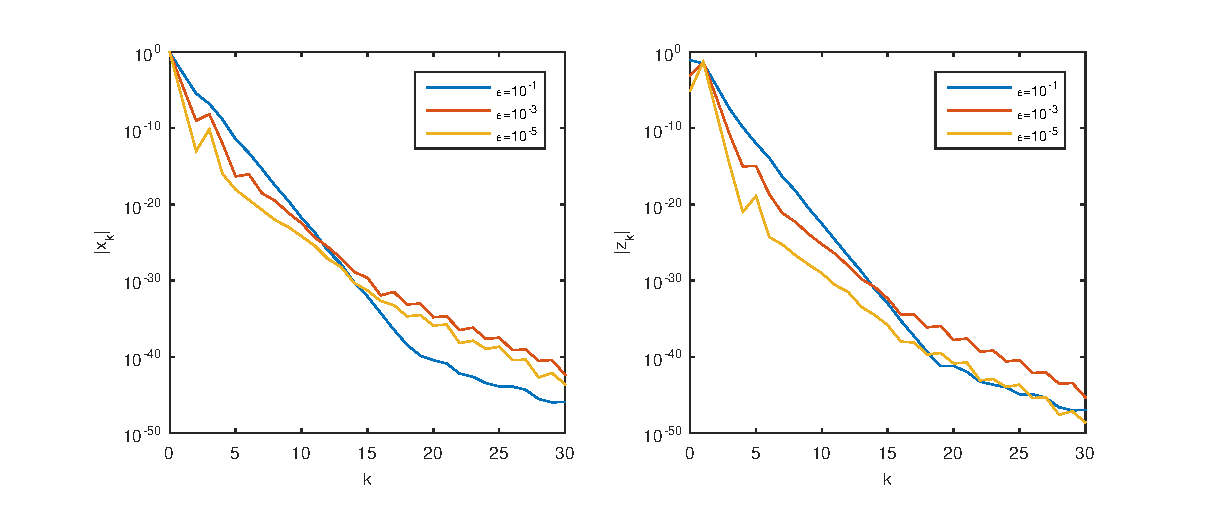
\includegraphics[width=1\textwidth]{img/chap3/norm_coeffs_series.eps}
\caption{Norme infinie des coefficients $(x_k\eeps)$ et $(z_k\eeps)$ en fonction de $k$ dans le cas \eqref{pb:edo_partic_1}.}
\label{fig:norm_coeffs_series}
\end{figure}
On voit alors qu'on peut choisir un rang maximal $k_{\max} = 20$ dans notre cas. Appliquons maintenant un schéma RK4 au polynôme $(u_k\eeps)_{0\leq k\leq 20}$ à $\dt$ fixé et pour diverses valeurs de $\epsilon$ pour étudier si le bon choix de coefficients suffit à diminuer la raideur du problème pour obtenir des schémas uniformément précis par défaut. 
\begin{figure}[!h]
\centering 
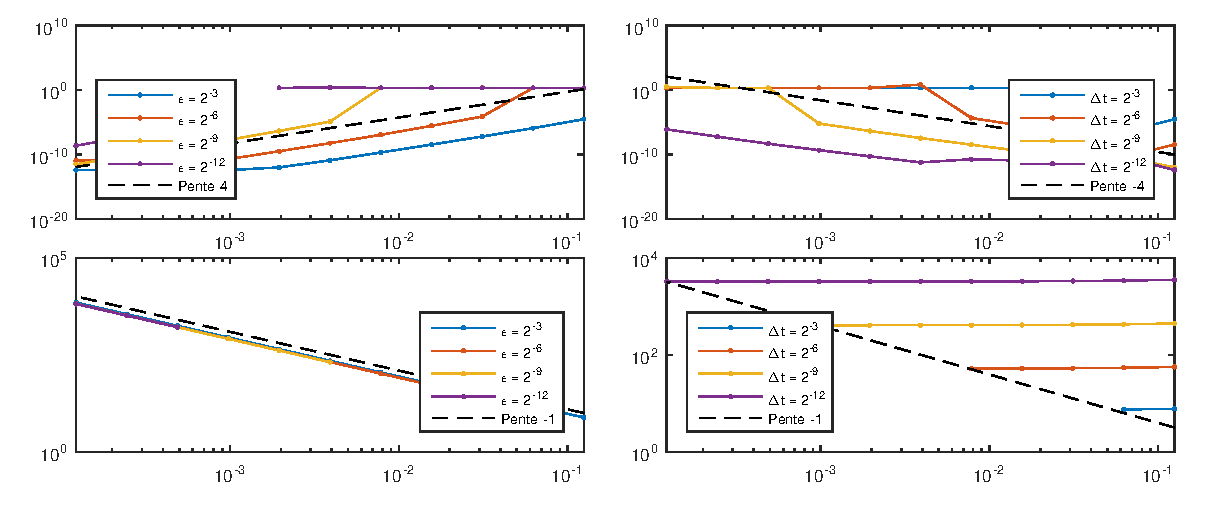
\includegraphics[width=\textwidth]{img/chap3/conv_rk4_series.eps}
\caption{Erreur relative en norme infinie sur $x$ (en haut) et erreur absolue en norme infinie sur $z$ (en bas) en fonction de $\dt$ (à gauche) et de $\epsilon$ (à droite) pour le cas \eqref{pb:edo_partic_1} avec un schéma RK4 sur les $(u_k\eeps)$.}
\label{fig:conv_series_cas1}
\end{figure}
On voit sur la figure \ref{fig:conv_series_cas1} que ce n'est absolument pas le cas, et que la convergence est la même qu'en considérant le système d'origine, sans séries. 
La stabilité est directement liée à $\dt/\epsilon$. 
On observe cela sur l'erreur de $z$ en fonction de $\epsilon$, où tracer une droite $\sim 1/\epsilon$ passe par le dernier point avant que la solution ne diverge pour différentes valeurs de $\dt$. 


\subsection{Implémentation par différences finies}

On voit qu'on peut restreindre l'ensemble de définition de $\tau$ à $[0,\Tk/\epsilon]$. Il faut donc discrétiser ce segment. 
Afin de profiter de la forme exponentielle des fonctions, on choisit une discrétisation de la forme 
$$ \tau_n = -C\ln(\xi_n) $$ 
avec $(\xi_n)_{0\leq n \leq N_{\tau}}$ une dicrétisation uniforme de $[e^{-\Tk/\epsilon},1]$ (décroissante pour avoir $(\tau_n)$ croissante), et $C$ une constante positive qui permet d'avoir une meilleure résolution sur les fonctions de base $(\tau\mapsto e^{-k\tau}), k\in\N$ et $(\tau\mapsto e^{-j\mu\tau}),j\in\N^*$. 
On choisit $C = \max(1/\mu,1)$ pour un bon compromis après une rapide étude de l'erreur d'intégration (avec la formule du trapèze) sur ces fonctions. \\

\subsubsection{Intégration du schéma}

On voit que la seule partie un peu difficile à implémenter pour le schéma sont les produit de convolution par $\tau\mapsto e^{-\mu\tau}$ et $\tau\mapsto e^{-(\mu+1)\tau}$. 
On approxime 

$$ \begin{array}{rl} \displaystyle
\int_0^{\tau_n} e^{-\mu(\tau_n-\sigma)}h(\sigma)d\sigma =& \displaystyle \sum_{k=0}^{n-1} \int_{\tau_{k}}^{\tau_{k+1}} e^{-\mu(\tau_n-\sigma)}h(\sigma)d\sigma \\
\simeq & \displaystyle \sum_{k=0}^{n-1} \left(\int_{\tau_k}^{\tau_{k+1}} e^{\mu(\sigma-\tau_n)} d\sigma \right)\frac{h(\tau_k)+h(\tau_{k+1})}{2}
\end{array} $$
soit pour le schéma, 
$$ Q_{\mu}[0]^{-1}h(\tau) \simeq \sum_{k=0}^{n-1} e^{-\mu\tau_n}(e^{\mu\tau_{k+1}}-e^{\mu\tau_k}) \frac{h(\tau_k)+h(\tau_{k+1})}{2}, $$
$$ S_{\mu}[0]^{-1}h(\tau) \simeq \frac{\mu}{\mu+1}\sum_{k=0}^{n-1} e^{-(\mu+1)\tau_n}(e^{(\mu+1)\tau_{k+1}}-e^{(\mu+1)\tau_k}) \frac{h(\tau_k)+h(\tau_{k+1})}{2}. $$

\begin{remark}
Si on voulait effectuer ce produit de convolution entre deux fonctions discrétisées, l'implémentation serait compliquée puisque la discrétisation n'est pas uniforme. 
En effet, dans le cas d'une discrétisation régulière on aurait 
$ \int_0^{\tau_n} a(\tau-\sigma)b(\sigma)d\sigma = \sum_{k = 0}^{n-1} \frac{\Delta\tau}{2} (a(\tau_n-\tau_k)b(\tau_k) + a(\tau_n - \tau_{k+1})b(\tau_{k+1})) + \O(\tau_n \Delta\tau^2)$ par règle du trapèze. 
Dans le cas d'une discrétisation non uniforme, on n'a pas forcément accès aux valeurs en $\tau_n-\tau_k$, ce qui rend cela impossible. 
\end{remark}

Une fois ces calculs faits, on implémente le schéma et on peut évaluer l'erreur. 

\subsubsection{Étude de l'erreur} \label{sec:err_loc_df}
On veut s'assurer que le schéma permet effectivement de résoudre le système \eqref{pb:EDO_var_cent} avec une précision uniforme. 
Pour cela, on calcule l'erreur pour diverses valeurs de $\dt$ et de $\epsilon$ sur le cas particulier \eqref{pb:edo_partic_1}, avec $N_{\tau} = 2^{10}$ (sachant que dans \cite{chartier2015UA}, la discrétisation est à $32 = 2^5$ points et les résultats sont bons). 

\begin{figure}[!h]
\centering\hspace*{-1.3cm}
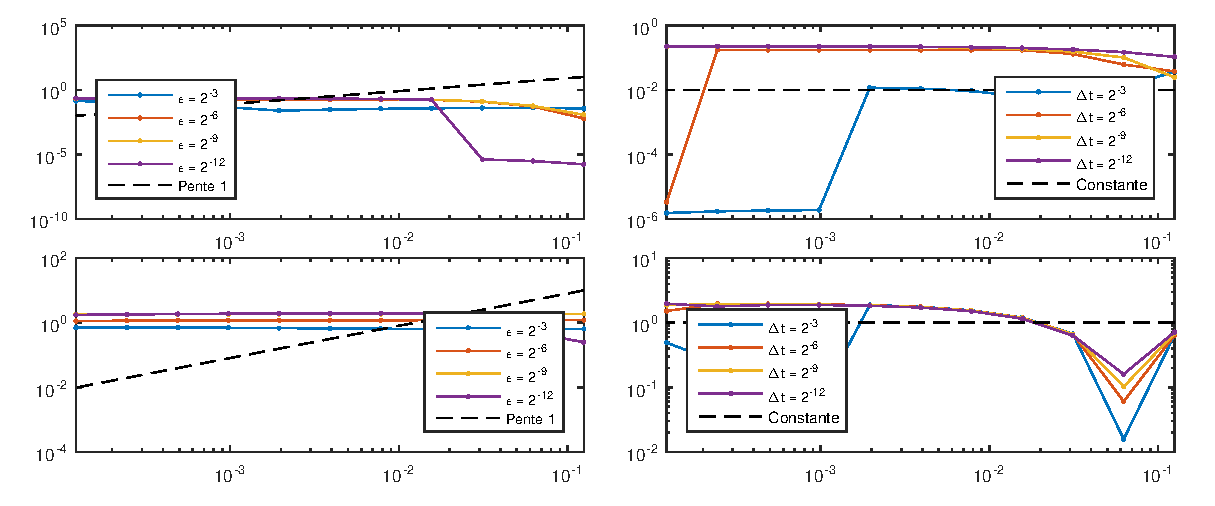
\includegraphics[width=\textwidth]{img/chap3/conv_rel_df_cas1.eps}
\caption{Erreur relative en norme absolue sur $x$ (en haut) et sur $z$ (en bas) en fonction de $\dt$ (à gauche) et de $\epsilon$ (à droite) pour le cas \eqref{pb:edo_partic_1} avec un schéma par différences finies.}
\label{fig:conv_interp_cas1}
\end{figure}

On voit sur la figure \ref{fig:conv_interp_cas1} que le nombre de points $N_{\tau}$ est insuffisant pour espérer avoir une quelconque convergence, malgré le fait qu'il soit élevé. 
On se rend compte que diminuer $\dt$ et $\epsilon$ nécessite d'augmenter $N_{\tau}$, ce qui rend l'utilisation de cette implémentation presque impossible : 
on peut avoir $\dt$ et $\epsilon$ arbitrairement faibles donc il n'est pas possible techniquement d'augmenter $N_{\tau}$ en accord ---et c'est absurde étant donné qu'on souhaite avoir une complexité indépendante de~$\epsilon$. 


\section{Implémentation avec la librairie \texttt{chebfun}}

Puisque l'approche par discrétisation n'a pas fonctionné, on décide d'utiliser la bibliothèque \texttt{chebfun}\cite{chebfun} sur \bsc{Matlab}. 
Cette bibliothèque utilise des interpolations par morceaux avec des polynômes de Chebychev pour effectuer des opérations quasi-exactes sur les fonctions. 
Son utilisation est simple et elle est très utile pour ce qu'on veut faire, mais on ne contrôle pas la complexité des opérations qui peut devenir très élevée dans le cas de fonctions raides. 

Cette fois-ci le calcul du produit de convolution se fait simplement avec la commande \texttt{conv}, ce qui rend l'implémentation aisée. 


\subsection{Erreur globale sur l'équation à variété centrale}

De même qu'avec les différences finies, on calcule l'erreur pour diverses valeurs de $\dt$ et de $\epsilon$ sur le cas particulier \eqref{pb:edo_partic_1}. 
\begin{figure}[!h]
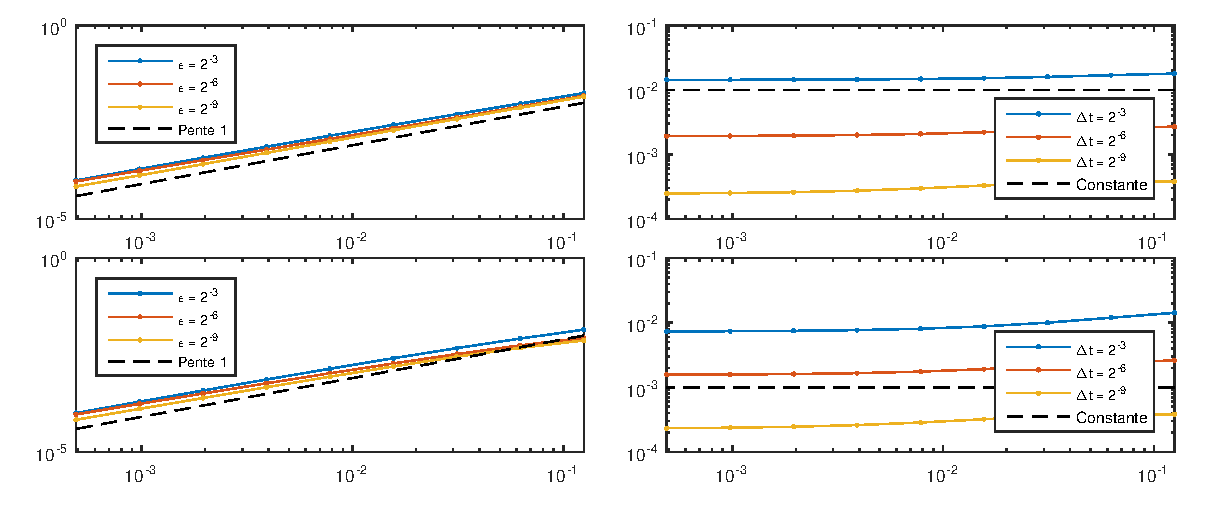
\includegraphics[width=\textwidth]{img/chap3/cheb/conv_rel_cheb_cas1.eps}
\caption{Erreur relative en norme infinie sur $x\eeps$ (en haut) et sur $z\eeps$ (en bas) en fonction de $\dt$ (à gauche) et de $\epsilon$ (à droite) pour le cas \eqref{pb:edo_partic_1} avec le schéma utilisant \texttt{chebfun}.}
\label{fig:conv_cheb_cas1}
\end{figure}

On voit que les résultats obtenus (en figure \ref{fig:conv_cheb_cas1}) sont ceux escomptés, à l'exception d'une légère perte d'ordre. 
On observe bien une convergence d'ordre 1 avec une erreur indépendante de $\epsilon$ comme assuré par le théorème \ref{thm:err_glob}. 
Observons le comportement sur un autre exemple, en choisissant $n=2,m=1$,

\begin{equation} \label{pb:edo_partic_2}
\left\{ \begin{array}{l}
f(x,z) = (1-z)\begin{pmatrix} 0 & -1 \\ 1 & 0 \end{pmatrix} x , \\
g(x,z) = x_1^2 x_2^2 \vphantom{\displaystyle\sum^0}
\end{array} \right. 
\qquad \text{et} \qquad 
\left\{ \begin{array}{l}
x_0 = \begin{pmatrix} 0,1 \\ 0,7 \end{pmatrix} , \\
z_0 = 0,05 . \vphantom{\displaystyle\sum^0}
\end{array} \right.
\end{equation}
%
On trace les mêmes courbes d'erreur en figure \ref{fig:conv_cheb_cas1}. 
\begin{figure}[!h]
\centering
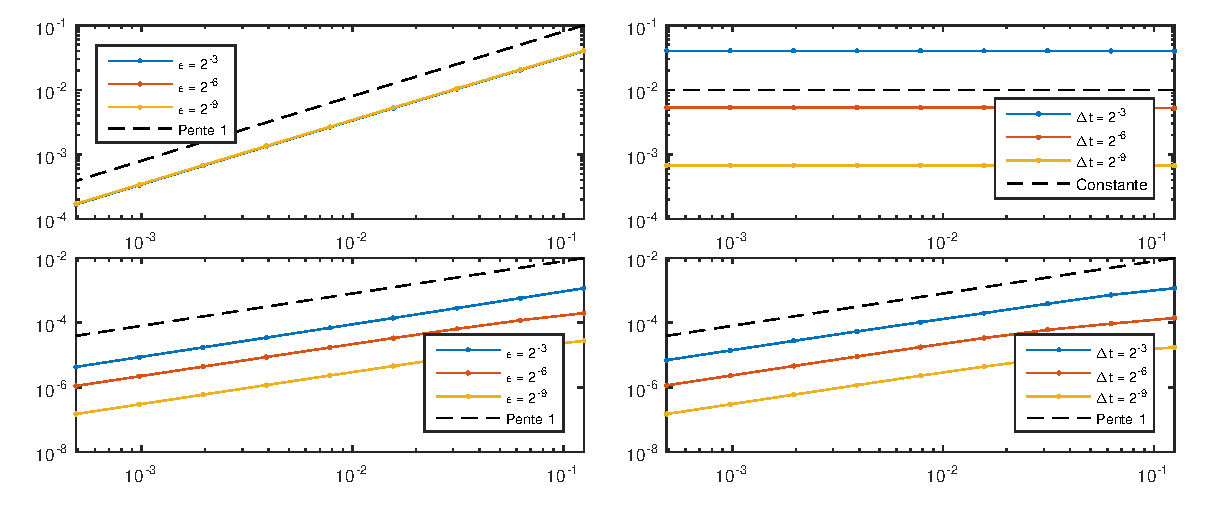
\includegraphics[width=\textwidth]{img/chap3/cheb/conv_abs_cheb_cas2.eps}
\caption{Erreur absolue en norme infinie sur $x$ (en haut) et sur $z$ (en bas) en fonction de $\dt$ (à gauche) et de $\epsilon$ (à droite) pour le cas \eqref{pb:edo_partic_2} avec le schéma utilisant \texttt{chebfun}.}
\label{fig:conv_cheb_cas2}
\end{figure}
Le schéma est uniformément précis d'ordre 1 pour le problème à variété centrale avec cette implémentation. 
On trace l'erreur absolue car la fonction $z\eeps$ s'annule en certains points et donc l'erreur relative est mal calculée, comme on le voit sur la figure \ref{fig:erreur_cheb_cas2}. 
\begin{figure}[!h]
\centering
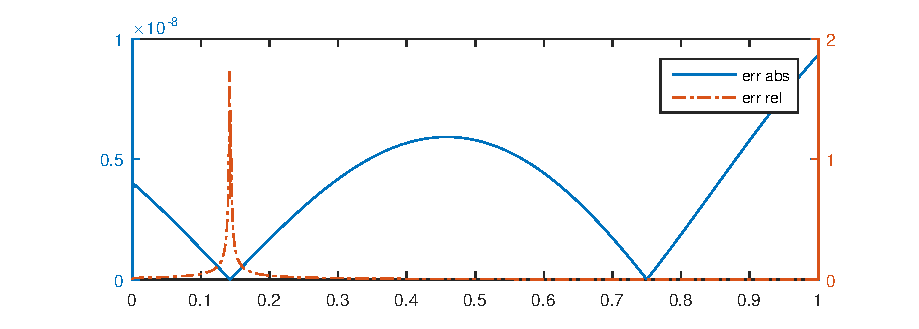
\includegraphics[scale=.85]{img/chap3/cheb/errors_cheb_cas2.eps}
\caption{Erreurs absolue (trait plein) et relative (pointillés) et leur échelle respectives à gauche et à droite en fonction du temps après calcul avec l'implémentation \texttt{chebfun} avec $\dt = 2^{-10}$ et $\epsilon = 2^{-14}$.}
\label{fig:erreur_cheb_cas2}
\end{figure}
Dans cet exemple, l'erreur relative, localisée sur un zéro, est d'ordre $1$ alors que l'erreur absolue est d'ordre $10^{-8}$. 
On voit néanmoins sur la figure \ref{fig:conv_cheb_cas2} que l'erreur absolue sur $z\eeps$ évolue en $\O(\epsilon\dt)$, ce qui est cohérent avec le fait que $z\eeps$ converge vers une fonction d'ordre $\epsilon$ en temps long. \\

Observons l'efficacité de cette approche utilisant \texttt{chebfun} sur les fonctions de $\tau$ directement, pour vérifier la robustesse de notre implémentation. 


\subsection{Erreur locale sur l'équation de transport}

On suppose que dans le premier cas test, les solutions obtenues avec \texttt{chebfun} sont exactes et on cherche à vérifier l'erreur locale en $\O(\dt^2)$.

On calcule de façon symbolique les fonctions $\tilde{X}\eeps(\dt,\cdot), \tilde{Z}\eeps(\dt,\cdot)$ obtenues après un seul pas de temps et on les compare à $X\eeps(\dt,\cdot),Z\eeps(\dt,\cdot)$ calculées avec notre schéma en utilisant un pas de temps $\dt_{qe} \ll \dt$. 
Si $X\eeps(\dt,\cdot),Z\eeps(\dt,\cdot)$ sont effectivement quasi-exactes, alors l'erreur sera d'ordre $\O(\dt^2)$. 

Pour le calcul symbolique, on passe par la transformée de Laplace puis la transformée inverse. 
On pourrait effectuer une intégration directe, mais cela permet d'introduire rapidement une nouvelle approche, qu'on pourra développer pour une autre implémentation après ce stage. 
En effet, puisque $\mathcal{L}\{\dptau h\}(\xi) = \xi \mathcal{L}\{h\}(\xi) - h(0)$, on a 
$$ \mathcal{L}\{X_1\eeps\}(\xi) + \frac{1}{\mu} \left( \xi \mathcal{L}\{X_1\eeps\}(\xi) - X_B(\dt) \right) = \mathcal{L}\{\dt f(X_0\eeps,Z_0\eeps) + X_0\eeps\}(\xi) $$
d'où 
\begin{equation} \label{eq:laplace_X}
\mathcal{L}\{X_1\eeps\}(\xi) = \frac{1}{\xi+\mu}\left( X_B(\dt) + \mu\mathcal{L}\{\dt f(X_0\eeps,Z_0\eeps) + X_0\eeps\}(\xi) \right) 
\end{equation}
et on peut appliquer une transformée de Laplace inverse pour obtenir $X_1\eeps$. De la même manière on a 
\begin{equation} \label{eq:laplace_Z}
\mathcal{L}\{Z_1\eeps\}(\xi) = \frac{1}{\xi+\mu+1}\left( Z_B(\dt) + \mu\mathcal{L}\{\dt g(X_0\eeps,Z_0\eeps) + Z_0\eeps\}(\xi) \right). 
\end{equation}

Avec cette approche, on est absolument certain que la solution numérique après un pas de temps est exacte. 
On effectue l'étude pour quelques valeurs $(\dt_i)$, la solution quasi-exacte étant calculé avec un pas de temps $\dt_{qe} = 2^{-10}\min(\dt_i)$. 

\begin{figure}[!h]
\centering
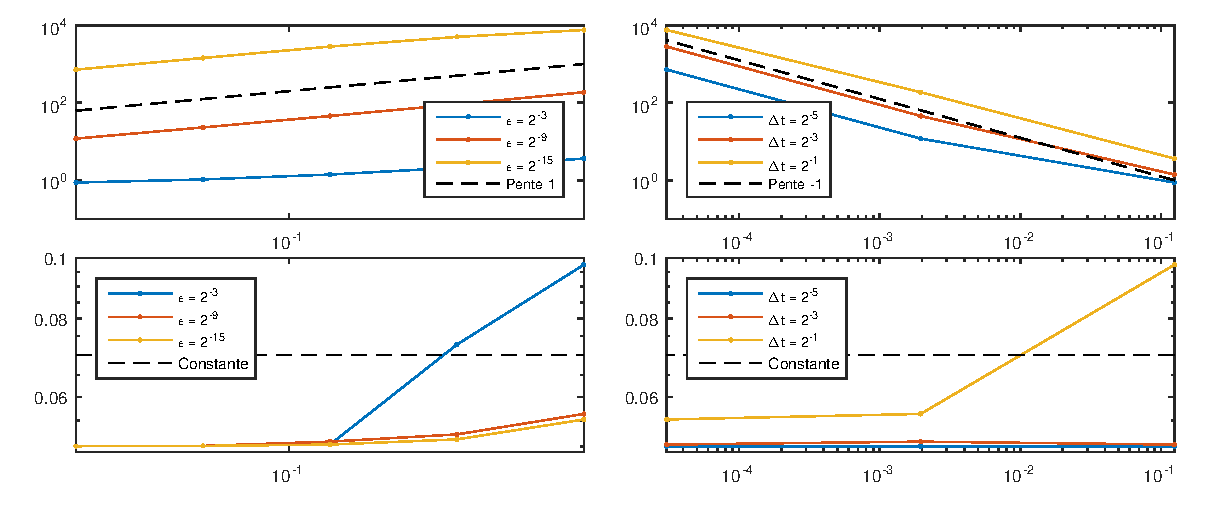
\includegraphics[width=\textwidth]{img/chap3/cheb/conv_cheb_one_step_cas1.eps}
\caption{Différence en norme $\Linftau$ entre la solution <<~quasi-exacte~>> calculée avec \texttt{chebfun} et la solution calculée symboliquement avec un seul pas de temps pour $X\eeps(\dt,\cdot)$ (en haut) et $Z\eeps(\dt,\cdot)$ (en bas) en fonction de $\dt$ (à gauche) et de $\epsilon$ (à droite).}
\end{figure}

On voit que le résultat n'est pas du tout celui auquel on s'attendait: on n'observe pas vraiment de convergence, l'erreur est toujours très grande, avec un plateau pour $\epsilon$ grand et $\dt$ petit. 
En outre, même pour $\dt,\epsilon$ grands, au lieu d'avoir une convergence en $\O(\dt^2)$ on observe une dépendance en $\O(\dt/\epsilon)$. 

Malheureusement, les temps de calcul sont très long et donc on ne peut pas effectuer les calculs avec $\dt_{qe}$ plus faible. 
Une observation plus précise des fonctions de $\tau$ calculées nous montre qu'elles deviennent de plus en plus raides en $\tau = 0$ au fil des itérations. 
On ne sait pas si cela est dû à l'implémentation ou au schéma directement. 
En effet, on n'a pas de relation pour évaluer $\|\dptau U_n\eeps\|$ en fonction de $n$, donc le schéma pourrait causer des fonctions difficiles à représenter numériquement, ce qui pourrait accentuer ce type d'erreurs. 

Cette interprétation n'explique cependant pas pourquoi l'erreur dépend de $\epsilon$. 
Probablement que le problème est accentué lorsque $\mu$ est petit. 

Étant donné que le schéma converge quand même pour la solution du système d'origine \eqref{pb:EDO_var_cent}, on peut se pencher sur les coûts et les conséquences liées à son implémentation dans un cadre <<~réel~>>.


\subsection{Coût de l'implémentation}

Notre implémentation n'est pas forcément très pratique, puisque la librairie \texttt{chebfun} est puissante mais coûteuse (en termes d'opérations), et elle n'est disponible que pour \textsc{Matlab}. 
On souhaite néanmoins en évaluer le coût opérationnel en fonction de $\dt,\epsilon$. Notre méthode est la suivante: 

\begin{itemize} 
\item On applique le schéma avec $\dt$ et $\epsilon$ fixés et on mesure le temps pris par les calculs. 
\item On mesure les erreurs absolue et relative sur $u = (x,z)$ grâce à une solution quasi-exacte calculée avec le schéma Radau IIA. 
\item On calcule une solution avec le schéma Radau en utilisant des tolérances absolue et relative de l'ordre des erreurs obtenues par le schéma et on mesure le temps de calcul. 
\end{itemize} 
Les calculs sont effectués sur un processeur Intel Core i5-6500U @ 2.30 GHz, à 2 c\oe{}urs. 
À notre connaissance, un seul processus était utilisé, même pour les opérations de \texttt{chebfun}. 
Cette procédure est répétée pour différentes valeurs de $\dt,\epsilon$ pour obtenir des courbes similaires à celles d'erreur en figure \ref{fig:cost_cheb_cas1}. 
\begin{figure}[!h]
\centering 
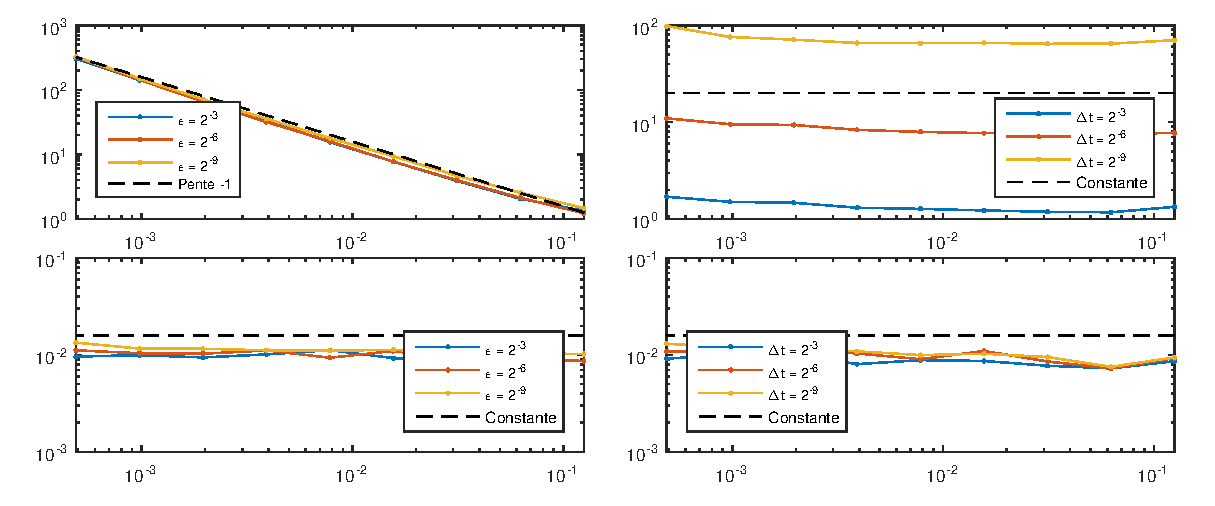
\includegraphics[width=\textwidth]{img/chap3/cheb/cost_cheb_cas1.eps}
\caption{Temps de calcul en secondes de la solution avec \texttt{chebfun} (en haut) et avec Radau IIA (en bas) en fonction de $\dt$ (à gauche) et de $\epsilon$ (à droite).}
\label{fig:cost_cheb_cas1}
\end{figure}

La première remarque qu'on peut faire est que le temps de calcul de la solution avec Radau IIA est toujours au moins 2 ordres de grandeur en dessous de celui pris pour notre schéma. 
On voit aussi que le temps de calcul avec Radau est presque indépendant de la tolérance (proportionnellement liée à $\dt$) et de $\epsilon$. 
On voit que le temps de calcul augmente un peu à mesure que $\epsilon$ diminue pour le schéma Radau et pour l'implémentation avec \texttt{chebfun}, mais de façon très faible. 

\section{Pistes de recherche}

Ce stage se poursuivant en thèse, il nous reste quelques idées à étudier plus profondément qu'on n'a pas encore pu développer. 

\subsection{Discrétisation du domaine de Laplace}

On a vu rapidement qu'on pouvait utiliser la transformée de Laplace pour résoudre le schéma numérique. Il y a quelques soucis liés à cette approche:
\begin{enumerate}
\item Le domaine de Laplace est de dimension 2, ce qui rend sa discrétisation plus coûteuse qu'en 1D,
\item La bibliographie autour de la transformée de Laplace numérique et son inverse est assez peu référencée, 
\item Les schémas impliquant cette transformée sont très rares, ce qui peut rendre l'approche difficile à accepter par la communauté, 
\item On a besoin d'un calcul direct et inverse rapide, avec une discrétisation de $[0,\Tk/\epsilon]$ adaptée pour pouvoir calculer $f(X_n,Z_n)$ et $g(X_n,Z_n)$ à chaque itération. Cela amène des questions : 
\begin{itemize}
\item Comment définir <<~adaptée~>>? 
\item Comment trouver une telle discrétisation de façon dynamique? 
\end{itemize} 
On a vu qu'une discrétisation fixe n'était pas adaptée au problème avec l'approche par différences finies.
\end{enumerate}
On voit ainsi que cette direction apporte de nombreuses problématiques à creuser, ce qui la rend à la fois attractive et difficile à aborder. 

L'argument principal en faveur de cette approche est que la transformée de Laplace peut être vue comme l'équivalent de la transformée de Fourier du cas périodique dont on s'inspire. 
En effet, la transformée de Laplace permettrait d'extraire facilement les coefficients d'une série $\sum_{k\geq 0} u_k e^{-k\tau}$ pour $\tau\in\R_+$ de la même manière que la transformée de Fourier avec les séries $\sum_{k\geq 0} u_k e^{-ik\theta}$ pour $\theta\in\R/P\mathbb{Z}$. 
Or on a vu qu'on pouvait essentiellement se ramener à des séries exponentielles pour résoudre le système \eqref{pb:EDO_var_cent}, ce qui permettrait peut-être de fabriquer des méthodes <<~spectrales~>> (il en existe pour le cas hautement oscillant). 


\subsection{Schéma local à coût plus faible}

Face à ce problème, on essaie d'appliquer un autre schéma, qui ne calcule pas $X\eeps,Z\eeps$ directement, mais qui peut peut-être servir pour $x\eeps,z\eeps$. 
L'idée est simple, même si l'étude théorique n'a pas été effectuée : il s'agit d'appliquer seulement la première étape du schéma, en boucle. Ainsi on pose 
$X_n\eeps(\tau) = x_n\eeps + \epsilon\int_0^{\tau} [f(x_n\eeps,e^{-\sigma}z_n\eeps) - f(x_n\eeps,0)]d\sigma$ et $Z_n\eeps(\tau) = e^{-\tau}z_n\eeps + \epsilon\int_0^{\tau} e^{\sigma-\tau} [g(x_n\eeps,e^{-\sigma}z_n\eeps) - \dpz g(x_n\eeps,0)\cdot e^{-\sigma}z_n\eeps]d\sigma$ et on peut calculer 
$$ x_{n+1}\eeps = e^{-\mu\dt/\epsilon} b_{\dt}^{(x)}(x_n\eeps,z_n\eeps) + \mu\int_0^{\dt/\epsilon} e^{-\mu(\dt/\epsilon - \sigma)} \big(\dt\, f(X_n\eeps(\sigma),Z_n\eeps(\sigma))+X_n\eeps(\sigma)\big) d\sigma $$
$$ z_{n+1}\eeps = e^{-(\mu+1)\dt/\epsilon} b_{\dt}^{(z)}(x_n\eeps,z_n\eeps) + \mu\int_0^{\dt/\epsilon} e^{-(\mu+1)(\dt/\epsilon-\sigma)} \big(\dt g(X_n\eeps(\sigma),Z_n\eeps(\sigma))+Z_n\eeps(\sigma)\big) d\sigma $$
où $b_{\dt}^{(x)}(x_n\eeps,z_n\eeps)$ et $b_{\dt}^{(z)}(x_n\eeps,z_n\eeps)$ donnent la valeur des conditions au bord calculées comme dans \eqref{eq:CB_XZ} en remplaçant $x_0,z_0$ par $x_n\eeps,z_n\eeps$, ces conditions au bord étant évaluées en $\dt$. 

En cas de convergence, cette approche permet une implémentation algébrique simple, au coût indépendant de $\epsilon$. 
En effet, ces nouvelles fonctions $X_n\eeps,Z_n\eeps,f(X_n\eeps,Z_n\eeps),g(X_n\eeps,Z_n\eeps)$ sont naturellement des séries exponentielles d'après leur définition, donc le seul cas particulier à considérer pour l'approche algébrique est $\mu\in\N$, ce qui n'est pas un frein. 

Le problème opérationnel de ce schéma est qu'il implique deux intégrations par pas de temps: une pour calculer $X_n\eeps,Z_n\eeps$ et une pour $x_{n+1}\eeps,z_{n+1}\eeps$. 
Ces intégrations étant simples, il semble plutôt efficace quand même. 
Cependant on aurait souhaité limiter le nombre d'intégrations étant donné que les schémas dans le cas hautement oscillant n'en effectuant qu'une par pas de temps. 

Néanmoins, ce schéma se présente comme assez simple à étudier théoriquement et à implémenter tout en pouvant fournir des résultats convaincants.
On a en effet pu l'implémenter très facilement en utilisant \texttt{chebfun} et on a observé une précision uniforme sur nos deux cas particuliers. 
Cela en fait une piste de recherche prioritaire. 


%\chapter{Présentation du problème et motivation} 

%%%%%%%%%%%%%%%%%%%%%%%%%%%%%%%%%%%%%%
% Exemple d'entrée dans le glossaire %
%%%%%%%%%%%%%%%%%%%%%%%%%%%%%%%%%%%%%%
%\newglossaryentry{FFT}
%{
%  name=FFT,
%  description={Fast Fourier Transform}
%}
%Utilisation de la \gls{FFT}


%%%%%%%%%%%%%%
% CONCLUSION %
%%%%%%%%%%%%%%
\chapterb{Conclusion}

On a présenté le modèle et les problèmes qu'il engendrait d'un point de vue numérique. 
On a ensuite effectué un développement double-échelle pour séparer la dynamique rapide $e^{-t/\epsilon}$ de la dynamique lente. 
Après cette séparation, on a exhibé des conditions nécessaires à la régularité du nouveau problème, et on a montré que sous ces conditions, le problème était bien posé. 
Une fois cela fait, on a trouvé des conditions initiales et au bord qui permettent d'assurer que $X,Z$ et leurs dérivées première et seconde en $t$ sont uniformément bornées. 
À partir de ces données, on a construit un schéma numérique uniformément précis qu'on a implémenté et dont on a évalué les performances et les limites en le comparant à d'autres approches moins coûteuses mais moins (voire pas) robustes. 
Les résultats étant insatisfaisant en termes de performance et d'exportabilité, on a rapidement présenté deux de nos pistes de recherche qui seront poursuivies en thèse. \\


Il est très facile de se perdre dans les différentes grandeurs en jeu dans ce problème: on a affaire à des séries en puissance de $\epsilon$ dont les coefficients sont des séries exponentielles en $\tau$, et on doit faire varier tout cela en fonction de $t$. 
On peut aussi facilement confondre régularité et caractère uniformément borné des dérivées, ce qui pose problème étant donné l'importance des conditions de compatibilité. 

Comme on l'a évoqué rapidement, il peut être intéressant de travailler avec des séries exponentielles, mais il n'est pas évident de construire une implémentation se basant uniquement là-dessus, et il faut se rendre compte que les coefficients en jeu sont plutôt instables ---d'où notre normalisation en section \ref{subsec:series}. 

Tous ces <<~pièges~>> sont autant de raisons qui ont rendu le début de ce stage un peu laborieux. 
Au bout d'un moment, la formalisation s'est mise en place et donc on a pu progresser relativement rapidement vers la fin. Les notions restent cependant complexes et nécessitent de prendre encore un peu de recul. \\


Le mélange d'algèbre, analyse, calcul formel et implémentations numériques de ce sujet est ce qui le rend tout à fait attirant pour une poursuite en thèse. 
Il est en outre apparent qu'il y a encore beaucoup de pistes à creuser en matière d'approche et d'implémentation et que donc ce sujet <<~préliminaire~>> à l'étude des EDP est déjà très intéressant en soi et motive à l'approfondir. 

%%%%%%%%%%%
% ANNEXES %
%%%%%%%%%%%
\appendix
\renewcommand{\chaptername}{Annexe}
%\addtocontents{toc}{\protect\renewcommand{\protect\chaptertitlename}{Ann. }
%\protect\setcounter{tocdepth}{0}}
\chapter{Présentation des cas tests}
\label{sec:ann_exemples}

\section{Équations scalaires couplées}

On rappelle le problème \eqref{pb:edo_partic_1}: \\
{\itshape{}Pour $\epsilon$ donné, trouver $x\in C^{\infty}([0,T]; \R$ et $z \in C^{\infty}([0,T])$ telles que} 
\begin{equation} \label{pb:ann_edo_partic_1}
\left\{ \begin{array}{l}
\dot{x} = -x^3(z-z^3/3) \vphantom{\displaystyle\sum_0} , \\ \displaystyle
\dot{z} = -\inveps z + x(1-z^2/2) 
\end{array} \right. 
\qquad \text{et} \qquad 
\left\{ \begin{array}{l}
x(0) = x_0 = 0,8 \vphantom{\displaystyle\sum_0} \\
z(0) = z_0 = 0,05 .
\end{array} \right.
\end{equation}
Traçons la solution de ce système sur $[0; 0,7]$ pour diverses valeurs de $\epsilon$. 
\begin{figure}[!h]
\centering
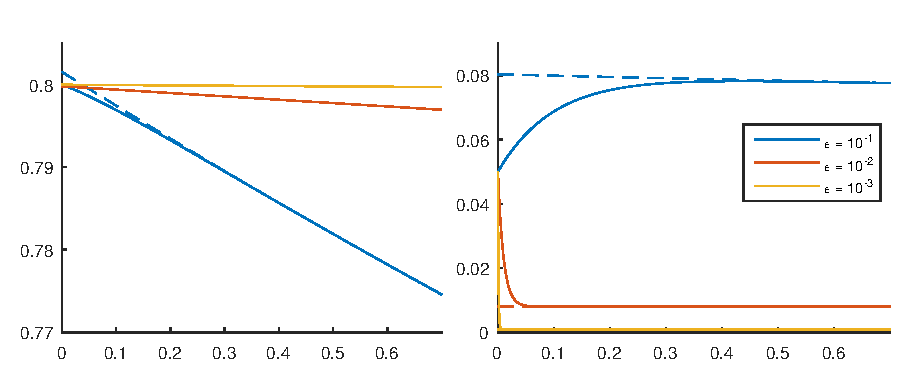
\includegraphics[width=.9\textwidth]{img/ann/solution_cas1.eps}
\caption{Solution $x$ (à gauche) et $z$ (à droite) du problème \eqref{pb:ann_edo_partic_1} sur $[0; 0,7]$, avec en pointillé l'approximation de la variété associée.}
\end{figure}

Il est apparent sur la figure qu'on a en temps long $\dot{x} = \O(\epsilon)$. 
On voit aussi très clairement $z_{\infty} = \O(\epsilon)$. 



\section{Oscillations lentes de $x$}

On rappelle le problème \eqref{pb:edo_partic_2}: \\
{\itshape{}Pour $\epsilon$ donné, trouver $x \in C^{\infty}([0,T];\R^2)$ et $z \in C^{\infty}([0,T]; \R)$ telles que} 
\begin{equation} \label{pb:ann_edo_partic_2}
\left\{ \begin{array}{l}
\dot{x} = (1-z)\begin{pmatrix} 0 & -1 \\ 1 & 0 \end{pmatrix} x , \\ \displaystyle
\dot{z} = \inveps z + x_1^2 x_2^2 \vphantom{\displaystyle\sum^0}
\end{array} \right. 
\qquad \text{et} \qquad 
\left\{ \begin{array}{l}
x(0) = x_0 = \begin{pmatrix} 0,1 \\ 0,7 \end{pmatrix} , \\
z(0) = z_0 = 0,05 . \vphantom{\displaystyle\sum^0}
\end{array} \right.
\end{equation}
On ne trace pas la solution en fonction du temps, mais plutôt son parcours dans $\R^3$. 
\begin{figure}[!h]
\centering
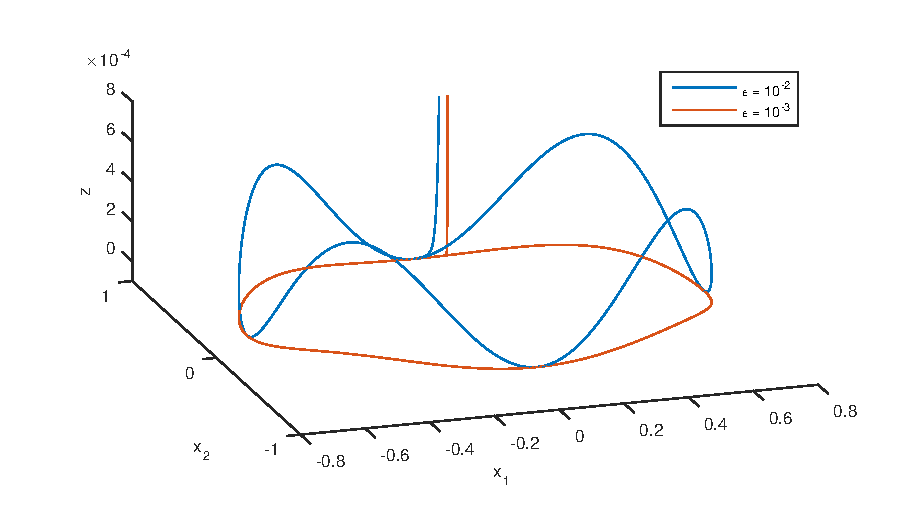
\includegraphics[width=.9\textwidth]{img/ann/solution_cas2.eps}
\caption{Parcours de $(x_1,x_2,z)$ dans $\R^3$ où $x,z$ sont solutions du problème \eqref{pb:ann_edo_partic_2} sur $[0; 10]$.}
\end{figure}

Le système semble converger rapidement vers un système périodique où $x_1,x_2$ et $z$ oscillent. 
On trace $z$ pour vérifier que la période ne dépend qualitativement pas de $\epsilon$.

\begin{figure}[!h]
\centering
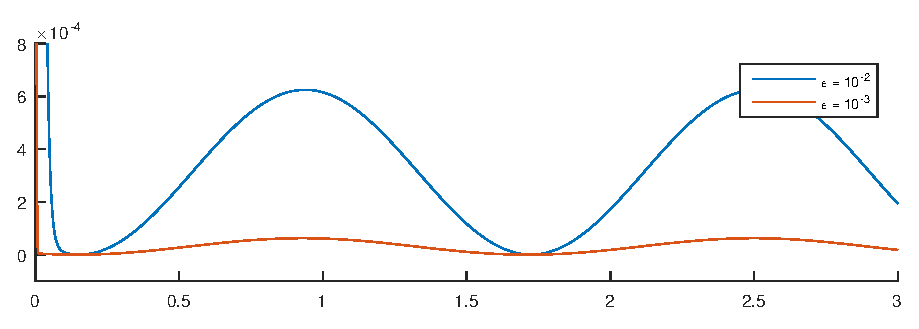
\includegraphics[width=.8\textwidth]{img/ann/solution_z_cas2.eps}
\caption{Solution $z$ du problème \eqref{pb:ann_edo_partic_2} sur $[0; 3]$ pour $\epsilon = 10^{-2},10^{-3}$.}
\end{figure}
En effet sur la variété on a $\dot{x} = \begin{pmatrix}
0 & -1 \\ 1 & 0 
\end{pmatrix} x + \O(\epsilon)$, ce qui cause l'oscillation de $x_1,x_2$. 
Le terme dominant pour déterminer la période est donc forcément indépendant de $\epsilon$. 
\chapter{Preuve du lemme \ref{thm:pb_gen_bien_pose} (p. \pageref{thm:pb_gen_bien_pose})}
\label{chap:ann_preuve}

On rappelle le problème \\
\textit{Trouver $(\overline{T},u)\in]0,T]\times C^0([0,\overline{T}]\times\R_+)$ tel que pour tout $(t,\tau)\in[0,\overline{T}]\times\R_+$ on ait }
\begin{equation} \label{pb:ann_trsp_u_no_eps}
\dpt u + \dptau u = F(t,\tau,u) 
\end{equation}
et le lemme qui assure qu'il est bien posé 

\newtheorem*{annlemma}{Lemme}
\begin{annlemma} 
Si $u_B\in C^0_b([0,T])$, $u_I \in C^0_b(\R_+)$ avec $u_B(t=0) = u_I(\tau = 0) =: u_0$, si $F$ est localement lipschitzienne par rapport à $u$, continue de $[0,T]\times\R_+\times E$ dans $E$, bornée par rapport à $\tau$, alors le problème \eqref{pb:ann_trsp_u_no_eps} est bien posé au sens suivant: 
 
Pour tout facteur $\kappa > 1$, il existe un temps $\Tk\in]0,T]$ tel que le problème \eqref{pb:ann_trsp_u_no_eps} a une unique solution $u$ dans $C^0([0,\Tk]\times\R^+)$, qui respecte l'inégalité 
\begin{equation}
\forall t\in [0,T_{\kappa}], \qquad \|u(t,\cdot) \|_{\Linftau} \leq \kappa\, \max\left\{ \|u_I\|_{\Linftau}, \|u_B\|_{\Linft} \right\}. 
\label{eq:ann_ineg_u_no_eps}
\end{equation}

Si en outre $F$ respecte $\forall (t,\tau,u)\in [0,T]\times\R_+\times E, |F(t,\tau,u)| \leq C_F |u| + D_F$ pour des constantes $C_F,D_F \geq 0$, alors il existe une unique solution $u$ dans $C^0([0,T]\times\R_+)$ qui vérifie 
\begin{equation}
\forall t\in[0,T], \|u(t,\cdot)\|_{\Linftau} \leq \left( \max\left\{ \|u_I\|_{\Linftau}, \|u_B\|_{\Linft} \right\} + t D_F \right) e^{t C_F}. 
\label{eq:ann_ineg_lin_u}
\end{equation}

\end{annlemma}

\begin{proof}
Intéressons nous aux droites caractéristiques du problème. 
\\
\begin{minipage}{.5\textwidth}
\begin{tikzpicture}
\begin{scope}[thick,decoration={
    markings,
    mark=at position 0.5 with {\arrow{>}}}
    ]
\node[inner sep=0pt,label=left:{0}] (O) at (0,0) {};
\node[inner sep=0pt,label=below:{$\tau$}] (tauf) at (7,0) {};
\node[inner sep=0pt,label=below:{$\tau_0$}] (tau) at (5,0) {}; 
\node[inner sep=0pt,label=left:{$t$}] (tf) at (0,5) {}; 
\node[inner sep=0pt,label=left:{$T$}] (T) at (0,4.5) {}; 
\node[inner sep=0pt,label=left:{$t_0$}] (t0) at (0,3) {};
\draw[<->] (tf) -- (0,0) -- (tauf); 
\draw[thick] (0,0) -- ++(4.5,4.5); 
\draw[dotted] (T) -- ++(7,0); 
\draw[dashed,postaction={decorate}] (t0) -- ++(1.5,1.5); 
\draw[dashed,postaction={decorate}] (tau) -- ++(2,2); 
\node at (4.5,3.8) {$t=\tau$};
\node at (2,3.5) {$\mathbb{U}_T$};  
\node at (4,1.5) {$\mathbb{L}_T$}; 
\end{scope}
\end{tikzpicture}
\end{minipage} \hfill
%
\begin{minipage}[t]{.48\textwidth}
\vspace*{-2.8cm}
Sous la diagonale $(t,t),\ t\in [0,T]$, la donnée initiale est en $(0,\tau_0), \tau_0\in\R_+$ et la droite est décrite par $(t,t+\tau_0)$. 
Au-dessus de la diagonale, elle commence en $(t_0,0)$ pour $t_0\in [0,T]$ et est décrite par $(t+t_0,t), t\in[0,T-t_0]$. 

\hspace{.5cm}Regardons d'abord le comportement de la solution sous la diagonale $(t,t)$. À partir d'une solution $u$, on pose $\phi(t,\tau) = u(t, t+\tau)$ la solution sur la caractéristique démarrant en $(0,\tau)$ qui respecte l'EDO
\end{minipage}
\begin{equation}
\dpt\phi(t,\tau) = 
F(t,t + \tau,\phi) \quad \text{ et }\quad \phi(0,\tau) = u_I(\tau) 
\label{eq:ann_pb_carac}
\end{equation} 
On sait que ce problème de Cauchy admet une solution unique locale sur $[0,t_m]$ (où $t_m > 0$ peut dépendre de $\tau$) par caractère localement lipschitzien de $F$. 

On peut mettre le problème \eqref{eq:ann_pb_carac} sous forme intégrale
$$ \phi(t,\tau) = \phi(0,\tau) + \int_0^t F(s,\tau+s,\phi(s,\tau))ds $$
pour $t \in [0,t_m]$. 
On cherche à déterminer un minorant de $t_m$ qui soit indépendant de $\tau$. 
Par inégalité triangulaire on obtient 
\begin{equation} 
|\phi(t,\tau)| \leq |\phi(0,\tau)| + \int_0^t |F(s,\tau+s,\phi(s,\tau))| ds.
\label{eq:ann_ineg_cauchy}
\end{equation}

Soit $\kappa > 1$, on pose $R = \max\left\{\|u_I\|_{\Linftau},\|u_B\|_{\Linft}\right\}$ et 
$$ M_{\kappa} = \sup \left\{ |F(t,\tau,u)| \ \big |\ (t,\tau,u)\in [0,T]\times\R^+\times E, |u|\leq \kappa R \right\}. $$
Par continuité et caractère borné de $F$, $M_{\kappa} < \infty$. Par définition, $|\phi(0,\tau)| \leq R$ et donc tant que $|\phi(t,\tau)| \leq \kappa R$ on a 
$ |\phi(t,\tau)| \leq R + t M_{\kappa} $
ce qui est assuré tant que $R + t M_{\kappa} \leq \kappa R$. 
Ainsi $\phi(t,\tau)$ est bien définie pour $t\leq\Tk$ avec 
\begin{equation} 
T_{\kappa} = \min \left\{ T, \frac{(\kappa - 1)R}{M_{\kappa}} \right\}
\label{eq:ann_def_Tk}
\end{equation}
qui vérifie toujours $T_{\kappa} > 0$. 
Sur $\mathbb{L}_{\Tk} := \{(t,\tau)\in [0,\Tk]\times\R_+,\ t\leq\tau\}$, on a $u(t,\tau) = \phi(t,\tau-t)$ et donc on peut définir une solution $u_{\mathbb{L}}$ sur le domaine réduit $\mathbb{L}_{\Tk}$. 

On remarque que $\phi(0,\tau)$ dépend continument de $\tau$ par continuité de $u_I$, et $F$ est continue par rapport à $t$ dans l'EDO sur $\phi(\cdot,\tau)$ donc la continuité se propage et $u_{\mathbb L}$ est continue sur $\mathbb{L}_{\Tk}$. 
\\

Au dessus de la diagonale, le problème est presque le même, on a $\dpt\varphi(t,t_0) = F(t + t_0, t, \phi)$, $\varphi(0,t_0) = u_B(t_0)$ pour $t_0\in[0,\Tk]$, d'où $|\varphi(t,t_0)| \leq |\varphi(0,t_0)|  + \int_0^t |F(s+t_0,s,\varphi(s,t_0))|ds$. 
La définition de $\Tk$ nous permet d'assurer de façon naturelle que $\varphi(\cdot,t_0)$ est bien définie sur $[0,\Tk-t_0]$. 
On peut alors définir une solution $u_{\mathbb{U}}$ sur le domaine réduit $\mathbb{U}_{\Tk} := \{(t,\tau)\in [0,\Tk]\times\R_+,\ t\geq\tau\}$ en posant $u_{\mathbb U}(t,\tau) = \varphi(\tau,t-\tau)$. 
Comme précédemment, la continuité de $u_I$ et de $F$ se propage et donc $u_{\mathbb{U}}\in C^0(\mathbb{U}_{\Tk})$. 

On peut maintenant procéder au <<~recollement~>> des solutions pour obtenir $u$ sur $[0,\Tk]\times\R_+$. On pose 
$$ u(t,\tau) = \begin{cases}
u_{\mathbb{L}}(t,\tau) & \text{ si } t\leq\tau \\
u_{\mathbb{U}}(t,\tau) & \text{ si } t > \tau 
\end{cases} $$

pour avoir $u$ solution du problème dans $L^{\infty}([0,\Tk]\times\R_+)$ et qui vérifie nécessairement l'inégalité \eqref{eq:ann_ineg_u_no_eps}. 
La continuité est assurée sur $\mathbb{L}_{\Tk}$ et sur $\mathbb{U}_{Tk}\setminus \{(t,t),\ t\in [0,\Tk]\}$, la seule difficulté est d'assurer la continuité de part et d'autre de la diagonale. 
Or on remarque que pour tout $t$ dans $[0,\Tk]$, on a l'égalité $\phi(t,0) = \varphi(t,0)$ puisque $\phi(\cdot,0)$ et $\varphi(\cdot,0)$ vérifient la même EDO avec la même condition initiale car $\phi(0,0) = u_I(0) = u_B(0) = \varphi(0,0)$, et la solution est unique sur $[0,\Tk]$. 
Ainsi $u_{\mathbb{L}}(t,t) = u_{\mathbb{U}}(t,t)$ et donc $u$ est continue de part et d'autre de la diagonale. 
Finalement, $u \in C^0([0,\Tk]\times\R_+)$. 
\\

Si on est dans le cas de $F$ bornée par une fonction affine, on applique le théorème de Grönwall à l'inégalité \eqref{eq:ann_ineg_cauchy} pour obtenir la relation \eqref{eq:ann_ineg_lin_u}, et le résultat de régularité est maintenu. 

\end{proof}
\chapter{Erreurs des schémas usuels}
\label{chap:erreus_schemas}

\section{Schémas à séparation des vitesses}
\label{sec:ann_schemas_sep_vitesses}

\subsection*{Schéma implicite-explicite}

On rappelle le schéma implicite-explicite
$$ \frac{1}{\dt}(x_{n+1}-x_n) = f(x_n,z_n) ,$$
$$ \frac{1}{\dt}(z_{n+1}-z_n) = -\inveps z_{n+1} + g(x_n,z_n) . $$

Pour étudier l'erreur locale on utilise la formule de Taylor à reste intégral 
$$ \begin{array}{rcl} 
\lex &=& x_1-x(\dt) = x_1 - x_0 - \dt f(x_0,z_0) - R^{(x)}_2(\dt) \\
&=& \displaystyle \int_0^{\dt} (t-\dt) \left[\dpx f(x,z)\cdot f(x,z) + \dpz f(x,z)\cdot \left(-\inveps z + g(x,z)\right) \right] dt 
\end{array}  $$
où $x,z$ sont évaluées en $t$ dans l'intégrande. 
Étant donné le comportement de la solution grâce au théorème de variété centrale (thm. \ref{thm:var_cent}), on peut supposer approximer $x(t) = x_0 + \O(\epsilon)$ et $z(t) = z_0 e^{-\alpha t/\epsilon} + \O(\epsilon)$. 
En se concentrant uniquement sur le terme en $e^{-\alpha t/\epsilon}/\epsilon$ dans l'intégrale et en majorant $\vertiii{\dpz f(x,z)}$ par une constante (indépendante de $\epsilon$), on obtient finalement 
$$ \lex = \O \left(\frac{\epsilon}{\alpha}(e^{-\alpha\dt/\epsilon} - 1 + \alpha\dt/\epsilon)\right), \qquad \epsilon,\dt \rightarrow 0^+ . $$
Ainsi avec $\dt \ll \epsilon$, on a $\lex = \O(\dt^2/\epsilon)$ et avec $\epsilon \ll \dt$ on a $\lex = \O(\dt)$. 

Sur $z$, on utilise directement la formule $z(\dt) = z_0 e^{-\alpha t/\epsilon}$ puisque le développement de Taylor ne traduit pas le comportement de la solution. On obtient alors 
$$ \lez = z_0 - z(\dt) = \left(\frac{1}{1+\dt/\epsilon} - e^{-\alpha\dt/\epsilon} \right)z_0 + \O(\epsilon). $$
Dans les faits on observe une convergence $\O(\dt^2/\epsilon^2)$ lorsque $\dt\ll\epsilon$, et $\O(\epsilon/\dt)$ quand $\epsilon\ll\dt$, ce qui suggère que la variété est bien approchée par le schéma (si bien que le terme $\O(\epsilon)$ n'a pas d'influence) et qu'on a $\alpha = 1$ (sinon la convergence $\dt\ll\epsilon$ serait $\O(\dt/\epsilon)$). 
\begin{figure}[!h]
\centering
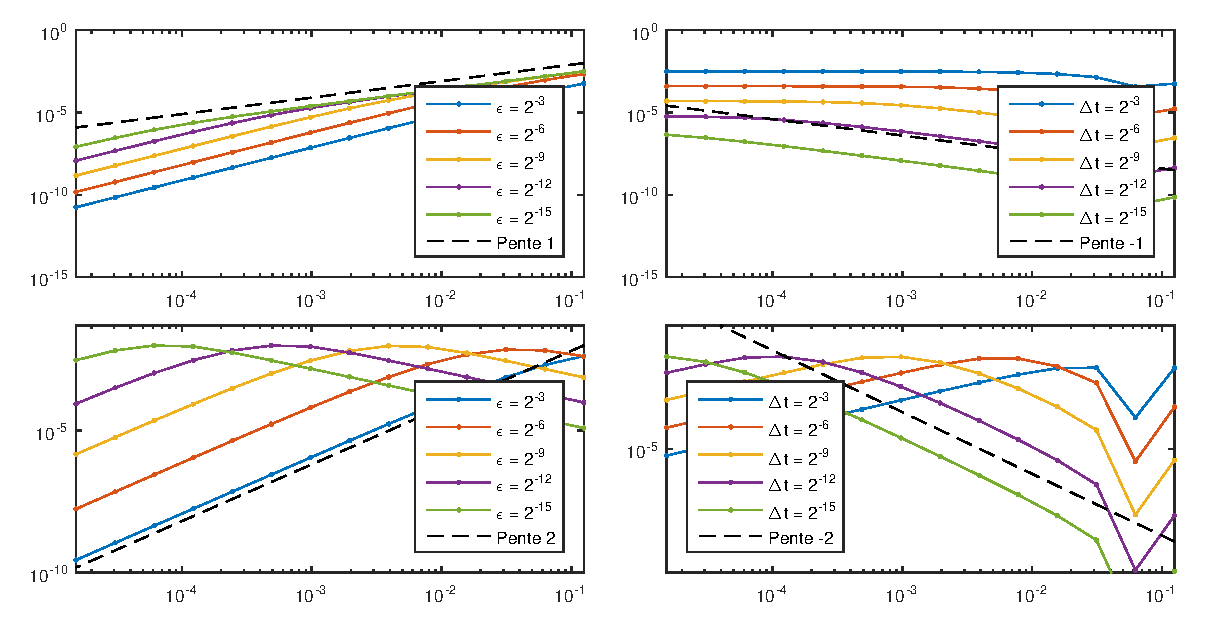
\includegraphics[width=\textwidth]{img/ann/conv_abs_imex_cas1.eps}
\caption{Erreur absolue en norme absolue sur $x$ (en haut) et sur $z$ (en bas) en fonction de $\dt$ (à gauche) et de $\epsilon$ (à droite) pour le cas \eqref{pb:edo_partic_1} avec un schéma implicite-explicite.}
\end{figure}

\subsection*{Splitting de Strang}

On peut calculer l'erreur avec le splitting de Strang dans le cas $f,g$ linéaires (pour pouvoir faire de l'algèbre d'opérateurs de façon simple). 
On sépare alors l'EDO $\dot{u} = -\inveps J u + Fu $ en deux systèmes $\dot{u} = -\inveps Ju$ et $\dot{u} = Fu$. 
L'erreur d'opérateur due au splitting est alors 
$$ e^{-\frac{\dt}{2\epsilon}J}e^{\dt F} e^{-\frac{\dt}{2\epsilon}J} - e^{\dt(-\inveps J + F)} = \frac{\dt^3}{4!} \left(\frac{1}{\epsilon^2}\big[[J,F],J\big] -\frac{2}{\epsilon}\big[ [J,F],F \big]\right) = \O\left(\frac{\dt^3}{\epsilon^2} \right). $$

Dans les faits on n'observe cette erreur que pour la variable $x$ et pas pour la variable $z$. 
En effet, sur nos exemples on a 
$$ \lex = \O\left( \dt^3/\epsilon^2 \right) , \qquad \qquad 
\lez = \O\left( \dt^2/\epsilon \right) . $$
\begin{figure}[!h]
\centering
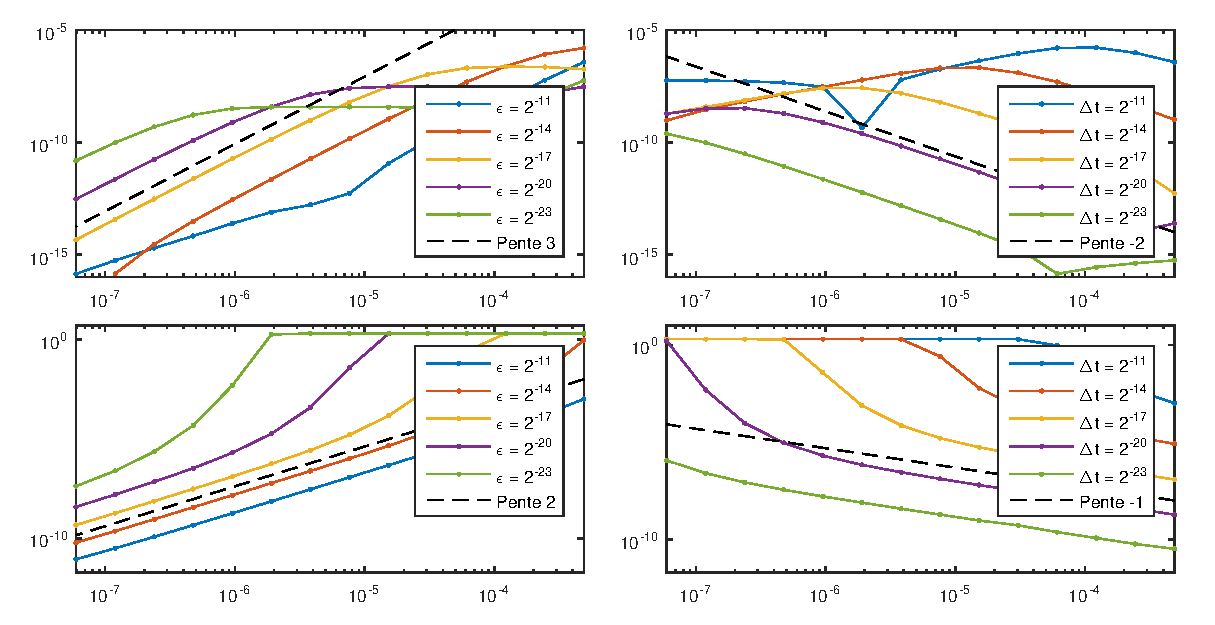
\includegraphics[width=\textwidth]{img/ann/conv_abs_strang_cas1.eps}
\caption{Erreur relative en norme absolue sur $x$ (en haut) et sur $z$ (en bas) en fonction de $\dt$ (à gauche) et de $\epsilon$ (à droite) pour le cas \eqref{pb:edo_partic_1} avec un splitting de Strang.}
\end{figure}

\section{Schéma à pas de temps adaptatif}
\label{subsec:ann_rke}

Expliquons le tableau de Butcher du schéma à pas de temps adaptatif. De manière générale, le tableau pour une méthode explicite imbriquée est 
\begin{center}
\begin{tabular}{c|ccccc}
    0    &     0    &          &    &    &    \\
  $c_2$  & $a_{21}$ &     0    &        &   &   \\
  $c_3$  & $a_{31}$ & $a_{32}$ &  0  &   &    \\
$\vdots$ & $\vdots$ &          &  $\ddots$ &  0  &   \\
  $c_s$  & $a_{s1}$ & $a_{s2}$ & $\cdots$ & $a_{s,s-1}$ &  0  \\ \hline
         & $b_1$  & $b_2$ & $\cdots$ & $b_{s-1}$ & $b_s$  \\ 
         & $\tilde{b}_1$  & $\tilde{b}_2$ & $\cdots$ & $\tilde{b}_{s-1}$ & $\tilde{b}_s$
\end{tabular}
\end{center}
On calcule alors les coefficients $k_s$ pour une EDO $\dot{u} = f(t,u)$ avec 
$$ \begin{array}{l}
k_1 = f(t_n,u_n), \\
k_2 = f(t_n+c_2\dt, u_n + (a_{21}\dt) k_1), \\
\quad \vdots \\
k_s = f(t_n+c_s\dt, u_n + \dt(a_{s1}k_1 + a_{s2}k_2 + \cdots + a_{s,s-1}k_{s-1}), \qquad\qquad\qquad\qquad\vphantom{0}
\end{array} $$
puis les deux estimations de la solution $\hat{u}_{n+1},\tilde{u}_{n+1}$ avec 
$$ \begin{array}{l}
\hat{u}_{n+1} = b_1 k_1 + b_2 k_2 + \cdots + b_s k_s , \vphantom{\displaystyle\int_0^1} \\
\tilde{u}_{n+1} = \tilde{b}_1 k_1 + \tilde{b}_2 k_2 + \cdots + \tilde{b}_s k_s .
\qquad\qquad\qquad\qquad\qquad\qquad\qquad\qquad\qquad\vphantom{\displaystyle\int_0^1}
\end{array} $$
Par convention, si le schéma avec $(b_i)_{1\leq i\leq s}$ est d'ordre $p$ alors celui avec $(\tilde{b}_i)_{1\leq i \leq s}$ est d'ordre $p-1$. 
Si $|\hat{u}_{n+1}-\tilde{u}_{n+1}| \leq Tol$ alors on admet le pas de temps $\dt$ et on pose $u_{n+1} = \hat{u}_{n+1}$. On estime $|\hat{u}_{n+1}-\tilde{u}_{n+1}| \leq |\hat{u}_{n+1}-u(t_{n+1})| + |\tilde{u}_{n+1}- u(t_{n+1})| = \O(\dt^{p+1}) + \O(\dt^p) = \O(\dt^p)$. 
On suppose alors $|\hat{u}_{n+1}-\tilde{u}_{n+1}| \simeq C \dt^p$ et $Tol \simeq C (\dt_{\text{opt}})^p$ (avec la même constante $C$ dans les deux relations), d'où l'adaptation de pas de temps 
$$ \dt \quad \longleftarrow \quad 0,9 \dt \left( \frac{Tol}{|\hat{u}_{n+1}-\tilde{u}_{n+1}|} \right)^{1/p} $$
le facteur $0,9$ étant appelé \textit{facteur de sécurité}. 

Dans notre cas particulier, on a 
\begin{center}
\begin{tabular}{c|ccccc}
 0  &  0   &  0  &  0  &  0  &  0  \\
1/3 & 1/3  &  0  &  0  &  0  &  0  \\
2/3 & -1/3 &  1  &  0  &  0  &  0  \\
 1  &  1   & -1  &  1  &  0  &  0  \\
 1  & 1/8  & 3/8 & 3/8 & 1/8 &  0  \\ \hline
    & 1/8  & 3/8 & 3/8 & 1/8 &  0  \\ 
    & 1/12 & 1/2 & 1/4 &  0  & 1/6
\end{tabular}
\end{center}
On implémente ce schéma et on mesure le temps de calcul et l'erreur en fonction de $\epsilon$ pour quelques valeurs de $Tol$. 
\begin{figure}[!h]
\centering
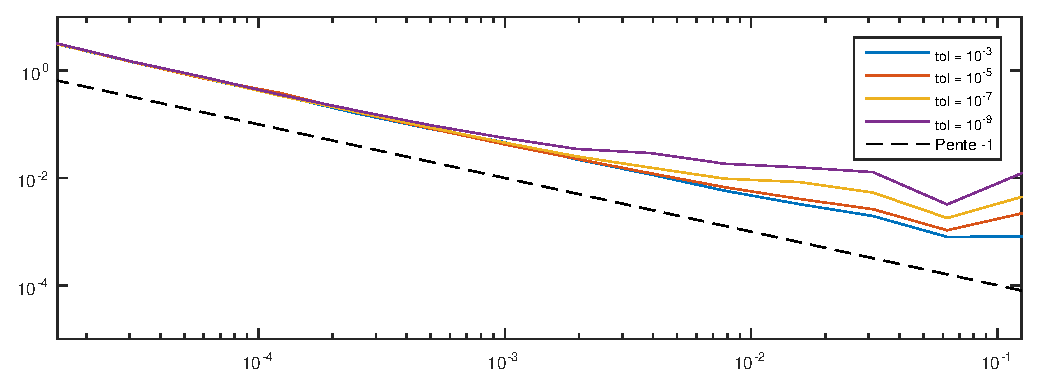
\includegraphics[width=.8\textwidth]{img/chap1/cost_rke.eps}
\caption{Temps de calcul (en s) avec notre méthode de Runge-Kutta imbriqués en fonction de $\epsilon$.}
\label{fig:cout_rke}
\end{figure}
\begin{figure}[!h]
\centering
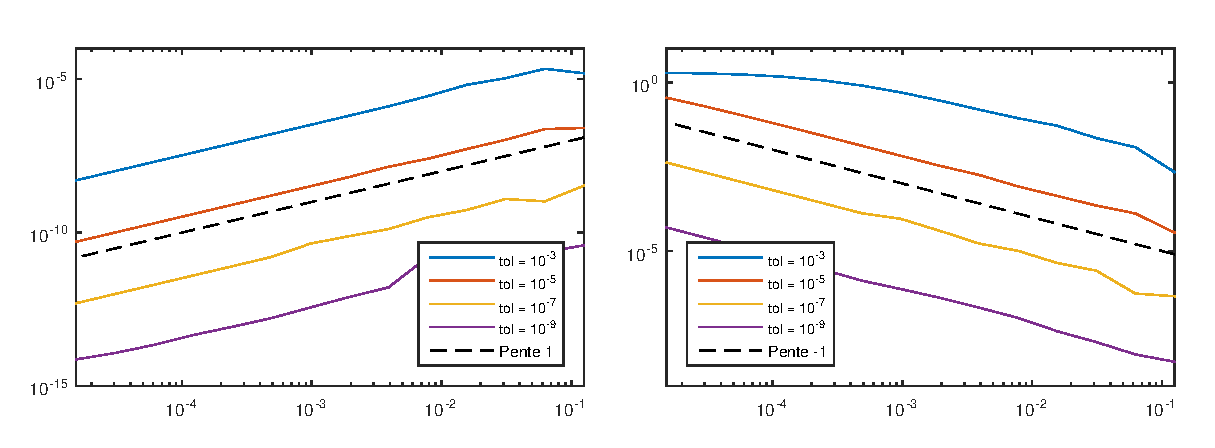
\includegraphics[width=\textwidth]{img/ann/conv_rel_rke.eps}
\caption{Erreur relative en norme absolue sur $x$ (à gauche) et sur $z$ (à droite) en fonction de $\epsilon$ pour le cas \eqref{pb:edo_partic_1} avec une méthode de Runge-Kutta imbriqués.}
\end{figure}

On voit alors que l'erreur sur $z$ augmente avec $\epsilon$ lorsque $\epsilon$ diminue, ce qui va à l'encontre de notre objectif. 
On rappelle en outre que le 

\section{Développement asymptotique}
\label{subsec:ann_asymp}

Dans \cite{castella2016formal}, on fournit les développement à l'ordre 3 en $\epsilon$ de la variété centrale $\epsilon h\eeps(\cdot)$ et de la condition initiale réduite $x_0\eeps$ dans les cas particuliers \eqref{pb:edo_partic_1} et \eqref{pb:edo_partic_2}. 
En particulier, dans le cas \eqref{pb:edo_partic_2}, on définit la variété tronquée et la condition initiale réduite tronquée 
\begin{align*}
\epsilon h^{[3]}(x) ={}& \epsilon x_1^2 x_2^2 - 2\epsilon^2 x_1 x_2(x_1^2 - x_2^2) + 2\epsilon^3 \left(x_1 x_2(x_1^2 - x_2^2 - 2) + (x_1^2 - x_2^2)^2 \right) \\
={}& \epsilon h\eeps(x) + \O(\epsilon^4), 
\end{align*}
\begin{multline*}
x_0^{[3]} = \left(1- \frac{\epsilon^2}{2}z_0^2 + \frac{\epsilon^3}{2} x_{0,1}^2 x_{0,2}^2 z_0 \right) x_0  
+ \Big[-\epsilon z_0 + \epsilon^2 x_{0,1}^2 x_{0,2}^2 \\
+ \epsilon^3 \left( \frac16 z_0^3 - 2(1+2 z_0)x_{0,1}x_{0,2}(x_{0,1}^2 - x_{0,2}^2) \right) \Big]
\begin{pmatrix} 0 & -1 \\ 1 & 0 \end{pmatrix} x_0 + = x_0\eeps + \O(\epsilon^4) .
%\qquad\qquad
\end{multline*} 

On définit la solution sur la variété approchée 
$$ \dot{x}^{[3]}_{\infty} = f(x^{[3]}_{\infty},\epsilon h^{[3]}\circ x^{[3]}_{\infty}), \qquad x^{[3]}_{\infty}(0) = x_0^{[3]} . $$
On peut alors la calculer et la comparer à la solution réelle en fonction du temps et on voit que l'écart diminue avec $\epsilon$. 
Vérifions que lors d'une simulation numérique, on obtient une erreur d'ordre $\O(\epsilon^4 + \dt^p)$ où $p$ est l'ordre de la méthode. 
L'erreur $\O(\epsilon^4)$ provient du modèle, de l'approximation de $x_0\eeps$ et $h\eeps$, tandis que l'erreur $\O(\dt^p)$ provient du calcul numérique de $x^{[3]}_{\infty}$. 

Pour la vérification, on commence par faire une résolution quasi-exacte sur la variété et sur le système initial pour vérifier la partie $\O(\epsilon^4)$, 
puis on fixe $\epsilon$ très faible et on résout le problème sur la variété approximée avec une méthode d'Euler explicite pour vérifier la partie $\O(\dt)$. 
Dans le cas \eqref{pb:edo_partic_1}, on a $\dot{x} = \O(\epsilon)$ sur la variété, donc cette approche est impossible 
(c'est pourquoi on utilise le cas \eqref{pb:edo_partic_2} pour ces tests). 

\begin{figure}[!h]
\centering
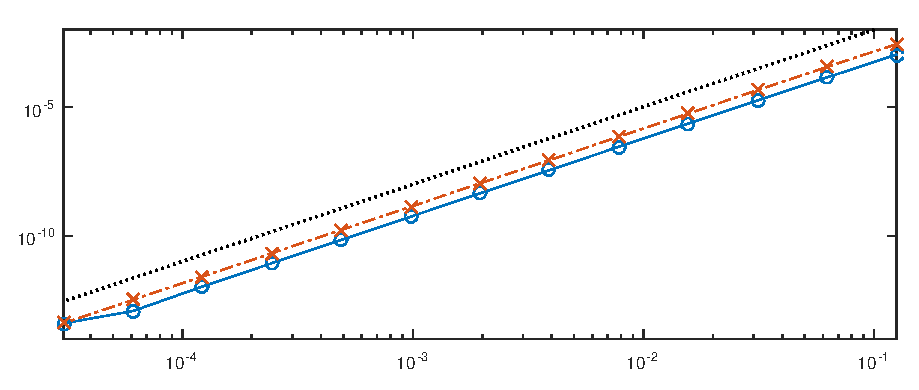
\includegraphics[width=.9\textwidth]{img/ann/erreur_manifold_approx.eps}
\caption{Différences entre $x\eeps$ et $x^{[3]}_{\infty}$ (ronds, trait plein bleu) et entre $z\eeps$ et $\epsilon h^{[3]}\circ x^{[3]}_{\infty}$ (croix, trait pointillé rouge) en fonction de $\epsilon$ en $t=1$, comparées à une pente $\epsilon^3$ (pointillés noirs) dans le cas test \eqref{pb:edo_partic_2}.}
\end{figure}
On voit alors que l'erreur est en $\O(\epsilon^3)$, ce qui n'est pas le résultat auquel on s'attendait. 
Il se peut que les formules de l'article soient erronées. 
En effet, en effectuant notre propre développement sur $h\eeps$ en remarquant $\dpz g = 0$, on obtient 
\begin{align*}
h\eeps(x) ={}& g(x,0) - \epsilon \dpx \left[ g(x,0) - \epsilon \dpx g(x,0)\cdot f(x,0) \right] \cdot f(x,\epsilon g(x,0)) + \O(\epsilon^3) \\
={}& g(x,0) - \epsilon \dpx g(x,0)\cdot f(x,0) + \epsilon^2 \dpx^2 g(x,0)\cdot (f(x,0),f(x,0)) 
\\ & + \epsilon^2 \dpx g(x,0)\cdot[ \dpx f(x,0)\cdot f(x,0) - \dpz f(x,0)\cdot g(x,0)] + \O(\epsilon^3) 
\end{align*} 
soit d'après nos calculs 
\begin{align*}
\epsilon h^{[3]}(x) ={}& \epsilon x_1^2x_2^2 - 2\epsilon^2 x_1x_2(x_1^2-x_2^2) + 2\epsilon^3 \left( x_1^2 x_2^2(x_1^3 x_2 - x_1 x_2^3 - 2) + (x_2^2-x_1^2)^2 \right). 
\end{align*}
Effectuer cette correction ne change pas les résultats, donc il se peut que la formule pour $x_0^{[3]}$ soit mal reportée dans l'article. 
On peut néanmoins vérifier la convergence en $\O(\dt)$ avec un schéma d'Euler explicite pour calculer la solution sur la variété approchée, dans le cas $\epsilon$ très petit (on choisit $\epsilon = 2^{-12}$). 
\begin{figure}[!h]
\centering
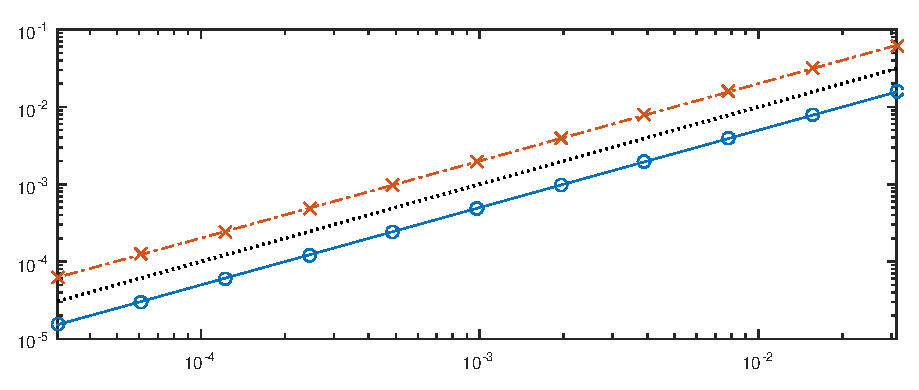
\includegraphics[width=.9\textwidth]{img/ann/erreur_manifold_euler.eps}
\caption{Différences entre $x\eeps$ et $x^{[3]}_{\infty}$ (ronds, trait plein bleu) et entre $z\eeps$ et $\epsilon h^{[3]}\circ x^{[3]}_{\infty}$ (croix, trait pointillé rouge) en fonction de $\dt$ en $t=1$ lorsque $x^{[3]}_{\infty}(1)$ est calculée par méthode d'Euler explicite de pas de temps $\dt$. La droite pointillée noire est de pente 1.}
\end{figure}

On voit alors que la convergence $\O(\dt)$ est bien vérifiée. 

%\addtocontents{toc}{\protect\renewcommand{\protect\chaptertitlename}{Ann. }}


%%%%%%%%%%%%%%%%%
% BIBLIOGRAPHIE %
%%%%%%%%%%%%%%%%%
\bibliographystyle{plain} %Ne pas modifier cette ligne
\bibliography{biblio} %L'argument doit etre le nom du fichier de la bibliotheque, sans l'extension .bib. Ici, mon fichier est biblio.bib



%%%%%%%%%%%%%%%%%%%%%%%%%%%%%%%%%
% LISTE DES FIGURES ET TABLEAUX %
%%%%%%%%%%%%%%%%%%%%%%%%%%%%%%%%%

\listoffigures
%\listoftables

%%%%%%%%%%%%%%%%%%%%%%
% INDEX ET GLOSSAIRE %
%%%%%%%%%%%%%%%%%%%%%%
% Mode d'emploi à cette adresse %
% http://www.tuteurs.ens.fr/logiciels/latex/makeindex.html
% http://www.xm1math.net/doculatex/glossaries.html
%\printindex
%\printglossaries



\end{document}